%%%%%%%%%%%%%%%%%%%%%%%%%%%%%%%%%%%%%%%%%%%%%%%%%%%%%%%%%%%%%%%%%%%%%%%%%%%%%%%%
%2345678901234567890123456789012345678901234567890123456789012345678901234567890
%        1         2         3         4         5         6         7         8

%\documentclass[letterpaper, 10 pt, conference]{ieeeconf}  % Comment this line out if you need a4paper

\documentclass[a4paper, 10pt, conference]{ieeeconf}      % Use this line for a4 paper

\IEEEoverridecommandlockouts                              % This command is only needed if 
                                                          % you want to use the \thanks command

\overrideIEEEmargins                                      % Needed to meet printer requirements.

%In case you encounter the following error:
%Error 1010 The PDF file may be corrupt (unable to open PDF file) OR
%Error 1000 An error occurred while parsing a contents stream. Unable to analyze the PDF file.
%This is a known problem with pdfLaTeX conversion filter. The file cannot be opened with acrobat reader
%Please use one of the alternatives below to circumvent this error by uncommenting one or the other
%\pdfobjcompresslevel=0

% See the \addtolength command later in the file to balance the column lengths
% on the last page of the document

% The following packages can be found on http:\\www.ctan.org
\usepackage{graphics} % for pdf, bitmapped graphics files
%\usepackage{epsfig} % for postscript graphics files
%\usepackage{mathptmx} % assumes new font selection scheme installed
%\usepackage{times} % assumes new font selection scheme installed
%\usepackage{amsmath} % assumes amsmath package installed
%\usepackage{amssymb}  % assumes amsmath package installed

\usepackage{graphicx}
\graphicspath{ {./graphics/} }

\usepackage{xcolor}
\usepackage{subcaption}

\newcommand{\ph}[1]{{\textbf{#1}:}} % paragraph header
\newcommand{\todo}[1]{{\color{red} #1 }} % Tasks to do
\newcommand{\inst}[1]{{\color{orange} #1 }} % instructions

\usepackage[normalem]{ulem}
\usepackage{url}
\usepackage{amsmath}
\usepackage{amsfonts}
\usepackage{amssymb}

\title{\LARGE \bf
NeBula Autonomy on Boston Dynamics Spot Robot: \\
Enabling Autonomous Exploration of Extreme Environments% Title consideration:
% 1. People can easily search "Autonomous Spot" and the paper will appear
% 2. A 2-4 noun words to recall: like Autnomous Spot in Challenging environment
}


\author{% <-this % stops a space
% \thanks{$^{1}$Albert Author is with Faculty of Electrical Engineering, Mathematics and Computer Science,
%         University of Twente, 7500 AE Enschede, The Netherlands
%         {\tt\small albert.author@papercept.net}}%
% \thanks{$^{2}$Bernard D. Researcheris with the Department of Electrical Engineering, Wright State University,
%         Dayton, OH 45435, USA
%         {\tt\small b.d.researcher@ieee.org}}%
}


\begin{document}


\maketitle
\thispagestyle{empty}
\pagestyle{empty}


%%%%%%%%%%%%%%%%%%%%%%%%%%%%%%%%%%%%%%%%%%%%%%%%%%%%%%%%%%%%%%%%%%%%%%%%%%%%%%%%
\begin{abstract}
This paper serves as one of the first efforts to enable large-scale and long-term autonomy using Boston Dynamics Spot robot. Motivated by exploring extreme environments and in particular underground environments in DARPA SubTerranean Challenge, this paper pushes the boundaries of the state-of-practice in enabling legged robotic systems to accomplish real-world complex missions in relevant scenarios. In particular, we will discuss the behaviors and capabilities which emerge from the integration of the autonomy framework NeBula (Networked Belief-aware Perceptual Autonomy) with next generation mobility systems. We will discuss the design, hardware, software challenges and solutions in mobility, perception, autonomy, and wireless networking, as well as lessons learned and future directions. We demonstrate the performance of the proposed system and solutions on physical systems in real-world scenarios, which achieved first place in the 2020 DARPA Subterranean Challenge Urban Circuit.
\end{abstract}
Video: Experimental results are available at ... 

%%%%%%%%%%%%%%%%%%%%%%%%%%%%%%%%%%%%%%%%%%%%%%%%%%%%%%%%%%%%%%%%%%%%%%%%%%%%%%%%
% \section{Instructions}
% \ph{Paragraph header} 
% \inst{Please start \uline{every single paragraph} with a paragraph header, summarizing the intention of that paragraph. This is mainly for iterations during the paper preparation. We can remove most of them for the final report.

% Graphs are available here for modification : 
% \url{https://docs.google.com/presentation/d/1dja02gUoBeNuNW-aHb6CmwaFevmf-jXMHk02NYbL1Ok/edit?usp=sharing}
% }
% {\color{red}fadnik means Fadhil or Nikhilesh}

% General Flow of the paper
% Introduction
% Architecture -> philosopy NeBula
% Mobility manager -> locomotion include from BD coauthor from them and sensors
% State Estimation -> Spot Frontend
% Perception Aware Planning -> Perception Aware Planning to Face Forward ..
% Experimental Result
% Lesson Learned  and Future:
% Recovery,
% Maybe stairs

% Conclusions



%%%%%%%%%%%%%%%%%%%%%%%%%%%%%%%%%%%%%%%%%%%%%%%%%%%%%%%%%%%%%%%%%%%%%%%%
\section{Introduction}\label{sec:intro}
%%%%%%%%%%%%%%%%%%%%%%%%%%%%%%%%%%%%%%%%%%%%%%%%%%%%%%%%%%%%%%%%%%%%%%%%
Robotically and autonomously mapping and traversing extreme environment under time constraints has a wide range of applications from search and rescue after natural disasters \cite{} to cave and extreme terrain exploration in planetary exploration \cite{}. In this paper, we discuss how bridging advanced locomotion capabilities and autonomy can address such complex missions. As a concrete mission, we focus on SubTerranean (SubT) Challenge \cite{subt_webpage} is a robotic competition that targets one such mission to explore, map, and search extreme underground environment. From mobility perspective, this mission imposes lots of constraints on the solution space. Some conflicting requirements imposed by elements of such extreme environment are 1) ability to carry large-enough payload that can enable  high-levels of sensing, autonomy, and computing, and communication capabilities, 2) endure long-term missions (at least 1 hour) and cover large areas (multi-kilometers), 3) to be small enough to go through passages as narrow as 80 cm in diameter, and 4) traverse mobility-stressing features, such as stairs, uneven terrains, obstacle-laden areas with high-risk regions. 
\begin{figure}[t!]
  \centering
  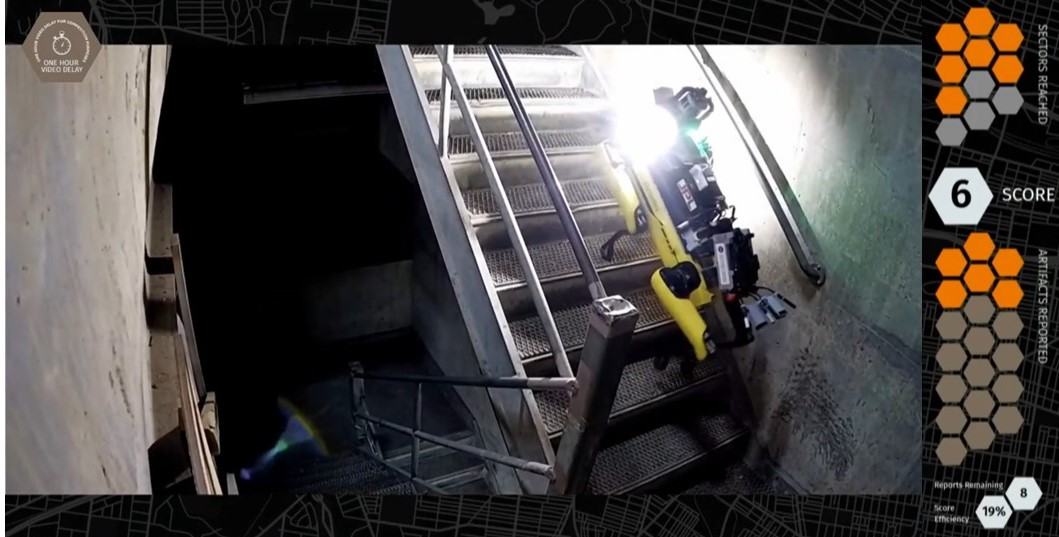
\includegraphics[width=0.5\textwidth]{spot_iros/graphics/spot_cover_ver1.jpg}
  \caption{This picture shows the NeBula-powered Spot robot climbing down four flights of stairs in the Urban Circuit of DARPA Subterranean challenge. This robot along with Team CoSTAR's other systems won this challenge.}
  \label{figurelabel}
\end{figure}

%\ph{Legged Mobility}
Legged robot offers unique mobility solutions that can adapt to various challenging environments. They have the potential to meet locomotion, payload, size, and endurance requirements of above-mentioned missions. \cite{whyrobotdeepmines}, Robosimian\cite{Karumanchi2017}, KAIST robot\cite{jung2018development}, Nimbro\cite{schwarz2017nimbro}, \cite{mit_cheetah}, \cite{bigdog}, \cite{Bellicoso2018}, \cite{miller2019tunnel} are just a few examples of such powerful systems. However, the research community is in the beginning of the road to enable these machines to autonomously carry out complex and full mission in extreme environments.

% \todo{fadil} \ph{Quadrupet real world applicationt: Anymal, Ghost, and Spot!}
% \inst{we should say great and positive things about Ghost and Anymal. and mention the state of practice in their autonomy...
% It should NOT be a "comparative paper". Instead of saying we are better, say that this is the "first autonomous behaviors in this scale on Spot". Compare the current results with the past results for Spot (rather than comparing with other platforms).}
% While various legged mobility solutions have been developed recently, 
% % Fadhil: cite 2-3 legged robot platform papers, 
% they have been minimally utilized  in  real-world  autonomous  applications\cite{whyrobotdeepmines}. 
% %
% One reported solution is an application of quadrupedal robot ANYmal in industrial inspection and search and rescue\cite{Bellicoso2018}.
% %
% In DARPA SubT Challenge, PLUTO team deployed multiple Ghost Robotics (GR) Vision 60 quadrupeds autonomously.\cite{miller2019tunnel}
% %
% While in industry world, Boston Dynamics' Spot, a direct successor to Big Dog\cite{bigdog}, shows impressive result in various applications(cite Spot web pages).
% %
% Recently, Boston Dynamic starts leasing their Spots to various industry and research communities to develop Spot application in real-world problems.

% % -Anymal: Anymal in real world application, Anymal‐toward legged robots for harsh environments. Advanced Robotics\cite{hutter2017anymal} 
% % - Ghost robotics: Upenn's Mine  Tunnel  Exploration  using  Multiple  Quadrupedal  Robots.

% % % another example
% % publicized work in 2008 . Recently they start collaborating.
% % How we expand Spot capability in extreme environment
% % emphasize our pioneer work in Spot autonomy

\begin{figure*}[h!]
  \centering
  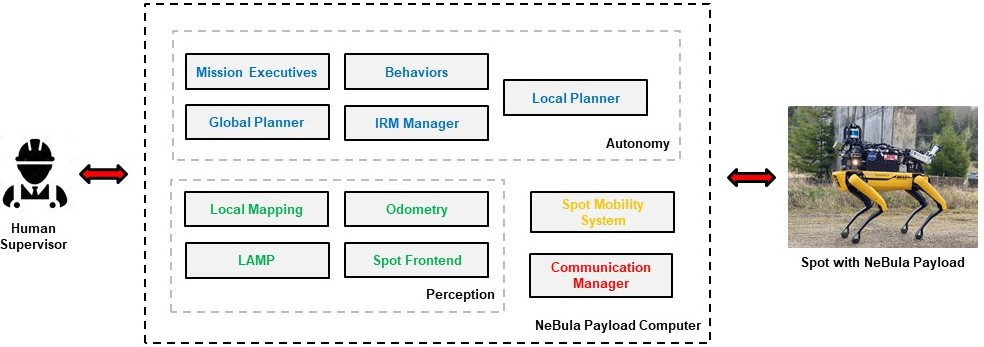
\includegraphics[width=0.8\textwidth]{spot_sa.jpg}
  \caption{\todo{fadnik} \inst{needs further update} Overview of software architecture to enable NeBula autonomy on Spot.}
  \label{fig:spot_sysarch}
\end{figure*}

%\ph{scope}
In this work, we focus on Boston Dynamics' Spot robot. We briefly discuss NeBula (Networked Belief-aware Perceptual Autonomy) framework and explain some elements of integrating full autonomy on the Spot robot. We describe the induced behaviors and performance of the system in a complex autonomous mission which led to the first place at the Urban Circuit of DARPA SubTerranean (SubT) Challenge. While the main objective of the paper is to provide a system-level overview of the entire autonomy stack and robot locomotion, we will describe in more detail some specific aspect of the algorithms that are critical to enable legged autonomy in complex missions. In particular, a few highlights of this paper and areas where we push the boundaries of the state-of-practice on Spot are:
\begin{enumerate}
    \item Enabling a legged platform to traverse more than 1km in a multi-level underground GPS-denied environment in less that 60 min with high-levels of autonomy
    \item \todo{fadnik-everyone} \inst{add more} Enabled a legged platform to traverse terrains with x amount of undulation and 3 levels
    \item \todo{fadnik-everyone} \inst{add more} enabled mapping of 3km cave networks with error less than 5m.
\end{enumerate}


%\ph{Outline}
In the next section, we describe the NeBula framework elements in high-level. In Section \ref{sec:spot} we discuss the robot locomotion and payload. Section \ref{sec:state_estimation}, \ref{sec:local_planning} and \ref{sec:mission_planning} focus on some specific algorithmic aspects on legged robot localization, perception-aware planning, and high-level mission planning. Experimental results are presented in Section \ref{sec:experiments} and we discuss lessons learned and future directions in Section \ref{sec:conclusion}.

%%%%%%%%%%%%%%%%%%%%%%%%%%%%%%%%%%%%%%%%%%%
\section{NeBula Autonomy}\label{sec:nebula}
%%%%%%%%%%%%%%%%%%%%%%%%%%%%%%%%%%%%%%%%%%%
Motivated by autonomously exploring extreme surface and subsurface terrains on Mars, Moon, and other planetary bodies, NASA's JPL is developing an autonomy framework, referred to as NeBula (Networked Belief-aware Perceptual Autonomy). The high-level objective of NeBula is to enable autonomously assessment and prediction of possible outcomes and risks in uncertain setting to enable a reliable coordinated multi-robot exploration of unknown and hard-to-access terrains.

To deal with unknown environments and uncertain setting, NeBula takes a probabilistic approach to model uncertainty. It takes the uncertainty into account to probabilistic fuse various sensing modalities, creates probabilistic representation of the robot knowledge of the environment, computes risk, and "proactively" plans to minimize the mission risk (similar to Markov Decision Processes). In Section ??, we will discuss ... and in Section ??, we will discuss some examples of how we incorporate sensing and perceptual uncertainties in the decision making process and create a perception-aware planning framework to reduce the risk prediction uncertainties.

% \todo{Ali} \ph{features} Long term goal for flight project
% CoSTAR related work:
% NeBula characteristic are ... Modular, Field hardened, ROS.

\ph{Architecture} Our autonomy framework NeBula consists of multiple components, which will be shortly described in the following.
Figure \ref{fig:spot_sysarch} provides a high-level overview of its architecture and how the modules are interconnected. The locomotion/sensing module encapsulates the dynamics models of the system, sensor models, and the API to send commands to the robot and read its sensory data. We will discuss this block further in Section \ref{sec:spot}. Odometry block captures algorithms to measure and estimate the relative motion of the robot. We will discuss some aspects of this block in Section \ref{sec:state_estimation}. This estimated odometry is then used within the front-end of our global SLAM system block. For details on the SLAM solution see \cite{Ebadi2020}. The planner block, includes the 1) mission planning layer that switch between various behaviors including exploration, stair-climbing, communication-recovery, etc. as well as 2) the global motion planning, and 3) low-level traversability planning. We will discuss these modules and highlight their uncertainty- and perception-aware aspects in Sections \ref{sec:mission_planning} and \ref{sec:local_planning}. The communication block is responsible for enabling data exchange between the multiple robots and a centralized server.


%%%%%%%%%%%%%%%%%%%%%%%%%%%%%%%%%%%%%%%%%%%
\section{Spot Mobility System}\label{sec:spot}
%%%%%%%%%%%%%%%%%%%%%%%%%%%%%%%%%%%%%%%%%%%
\ph{Locomotion system} 
Spot is a quadrupedal robot developed by Boston Dynamics to provide mobility in extreme environments and conditions. Spot can traverse various terrain types, including grass, sand and gravel at slopes of up to $\pm$30~deg. %Spot can operate in a wide range of temperatures (-20~C to 45~C), in light rain and in ambient lighting down to 2~Lux. 
It has separate gaits for dynamically stable movement, uneven terrain and stair climbing. %Spot can carry external payloads in excess of 14~kg operates for 90~minutes  (mixed usage). 

%NeBula has the ability to autonomously command Spot's locomotion in several aspects.

% It can carry about 14 kg of payload and it lasts about 90 min. Boston Dynamics offers a wide range of low--level motion planning algorithms. The developer can use the Boston Dynamic API to access internal sensor and map data and also send velocity of waypoint commands for the internal planner.

\ph{Sensing system} NASA JPL's NeBula Sensor Package (NSP) is designed with consideration for Spot’s overall traversability capabilities, mechanical constraints, and the sensor requirements of NeBula autonomy (Fig. \ref{fig:spot_full_nebula_form}). Spot's perception package from Boston Dynamics comprises five custom Realsenses distributed around the vehicle. The Nebula Sensor Package includes a VLP16 LIDAR, three D435i Realsenses, three high intensity LED's, a FLIR thermal camera, and the shock absorbing, rigid mechanical structure. Spot is a fast moving quadruped with the ability to traverse rough terrain. With NeBula autonomously driving this capability to its limit, the NSP can experience significant forces, moments, and vibrations. A combination of hard resin urethane, semi rigid carbon infused nylon and aluminium are used in the manufacturing process for increased rigidity and lightweight build. %As Spot is being used with NeBula as a research platform while pushing the envelope of the current state of the art of autonomous systems, 
Further, the design takes into consideration atypical load paths for shock absorption during falls. %Furthermore, the  sensor package needs to be adaptable to changing requirements. This is pertinent when competing in a DARPA challenge where the understanding of the competition and environment is rapidly evolving.
%\begin{figure}[h!]
%  \centering
%  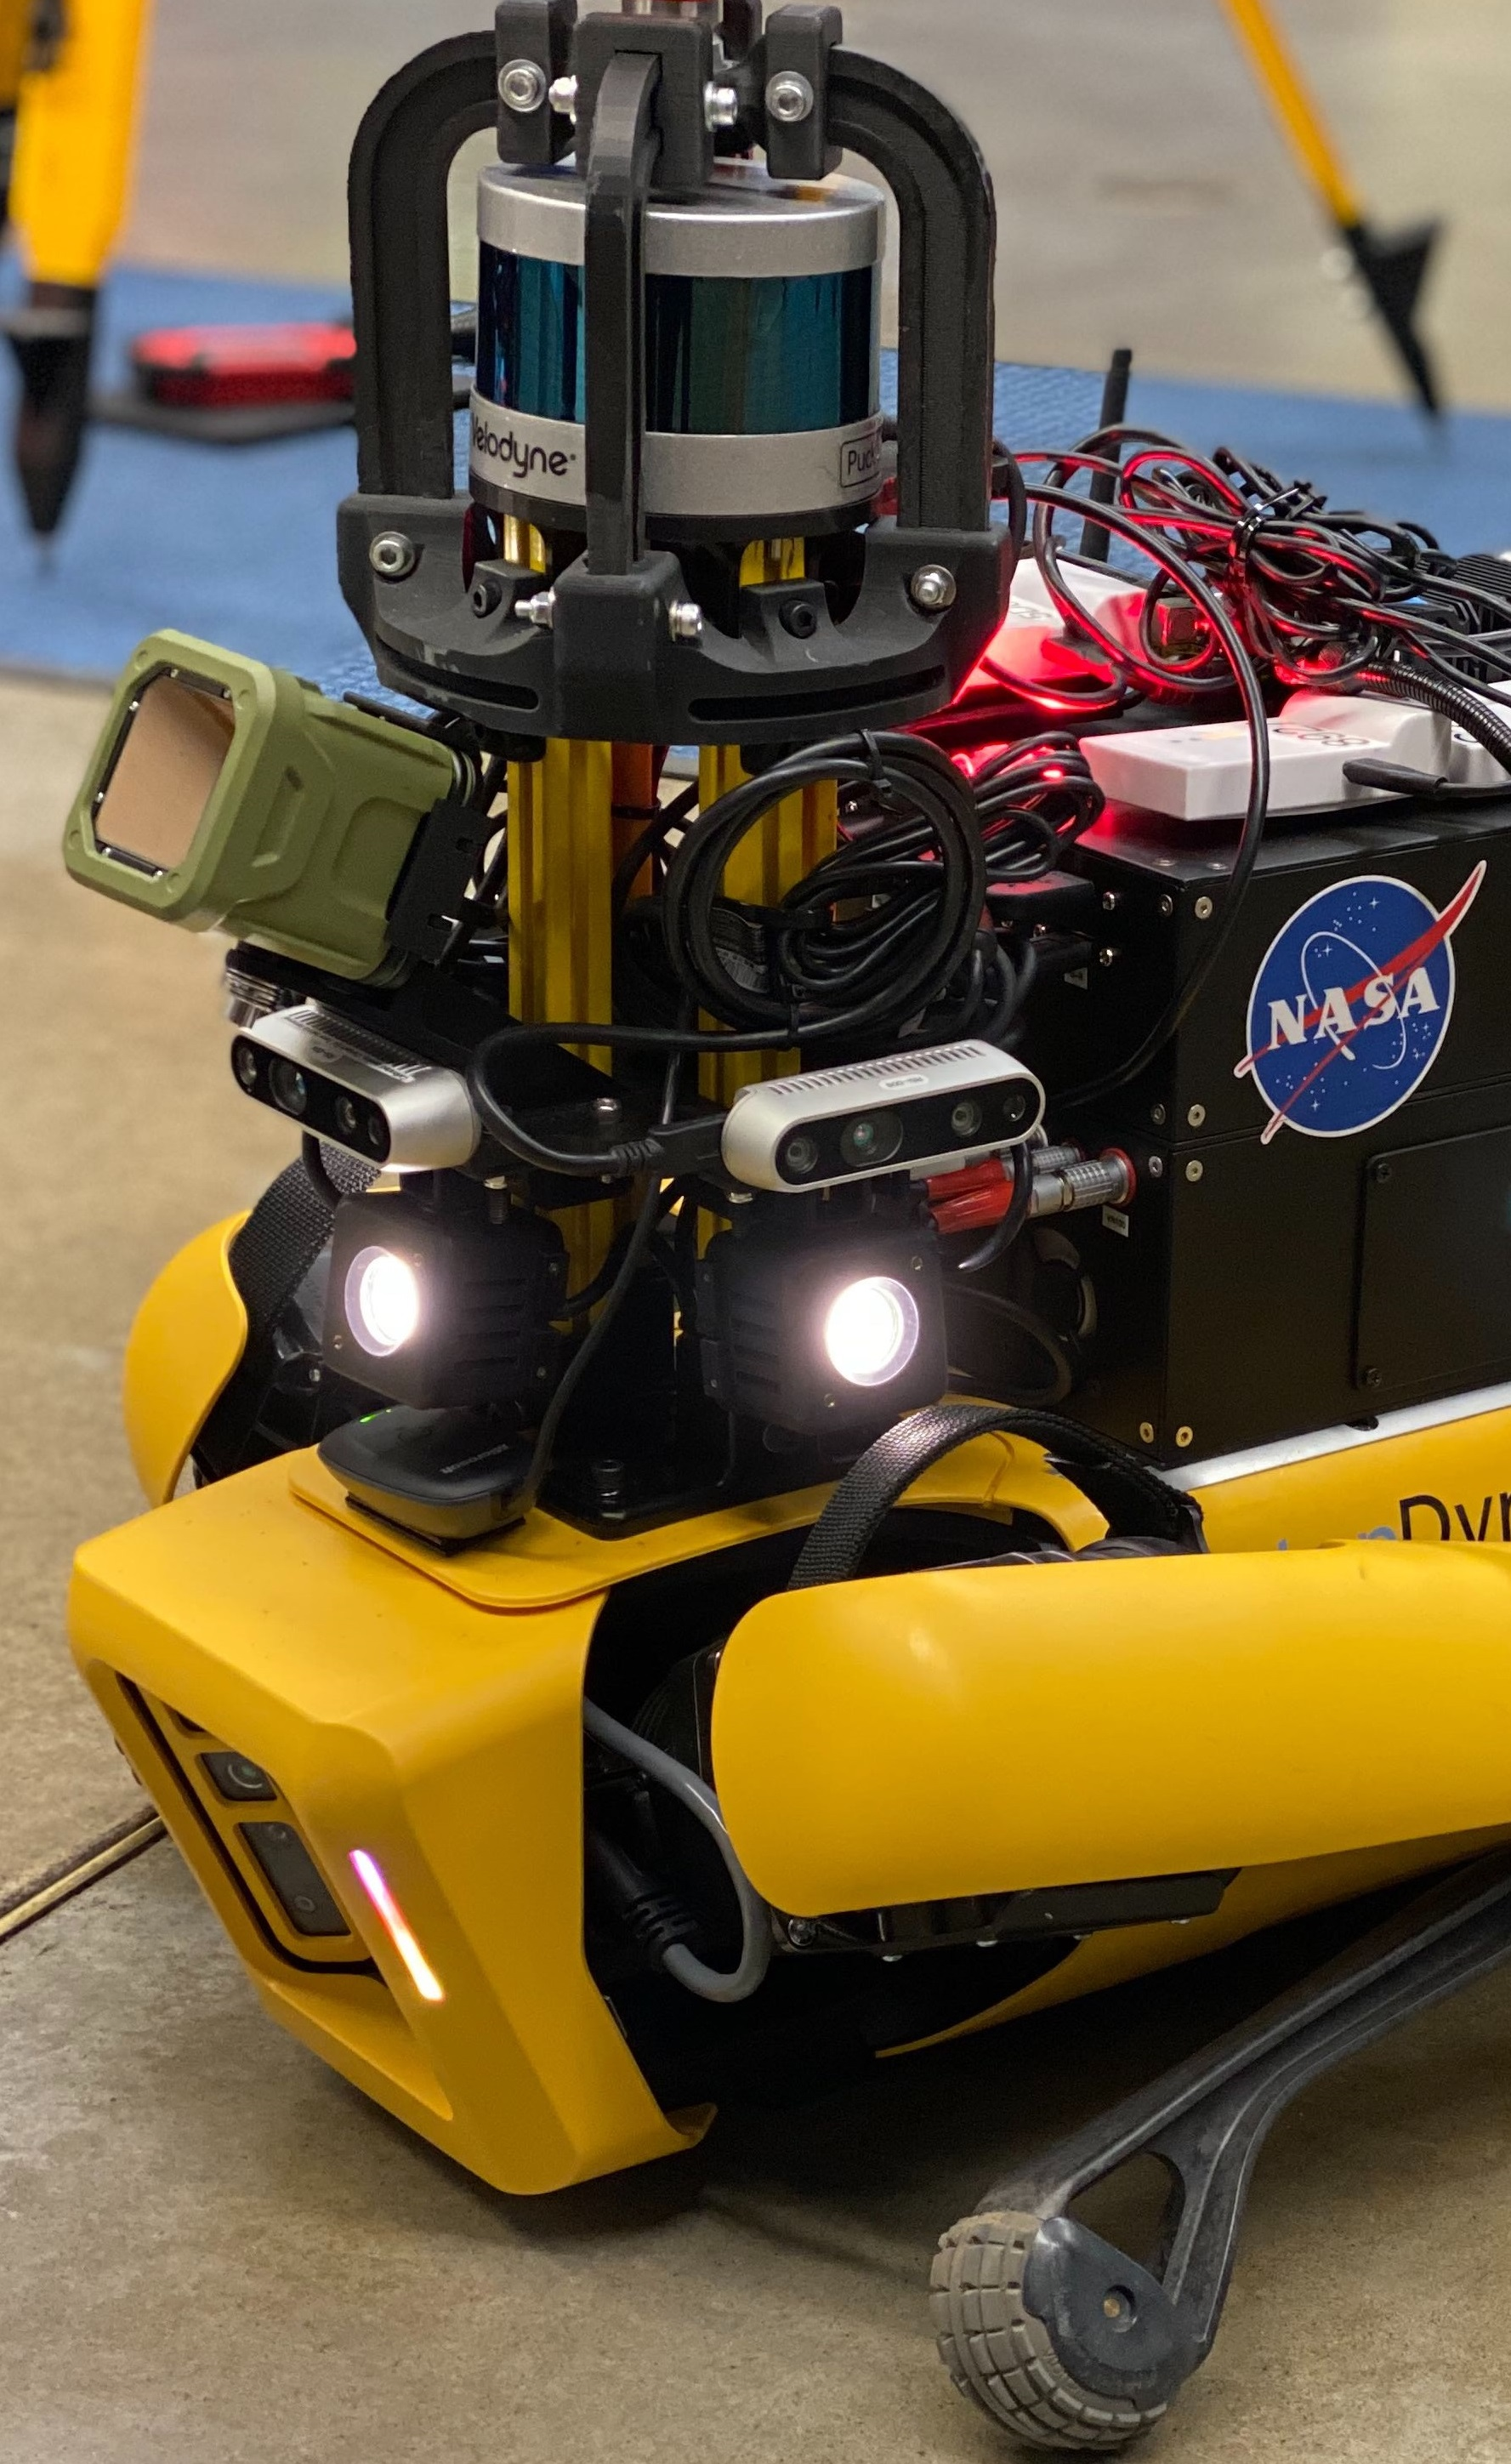
\includegraphics[width=0.2\textwidth]{spot_iros/graphics/spot_sensor_package_NSP_2.jpg}
%  \caption{Spot with Nebula Sensor Package Mounted}
%  \label{fig:spot_payload}
%\end{figure}

\ph{Power and Computing}
NASA JPL's NeBula Power and Computing Core (NPCC) is designed to mount onto Spot as an auxiliary payload which provides power to all of the sensors and the computers used for autonomy. The payload enclosure is designed with Aluminum to provide protection to the internal electronics if Spot were to fall. The payload is powered from an external lithium high capacity battery to provide isolation and extended battery life for the Spot internal battery. The NPCC also features a custom JPL power distribution and safety module, which provides fuses, overcurrent protection, overvoltage protection, inrush current limiting and power sequencing of five high efficiency voltage regulators for the sensors, lights and computers. %In addition, the power module manages the physical and remote e-stops and safety systems for the vehicle. Communication to the human supervisor is achieved using a Silvus Technologies Streamcaster radio. High bandwidth communication between the computers, radio, LIDAR and Spot is done through Ethernet via an internal network switch. The cameras, IMU and UWB modules interface to the computers via USB through multiple powered hubs. 
The payload uses two high level computers (Intel NUC and NVidia Xavier) for mission autonomy and semantic scene understanding.

\begin{figure}[thpb]
  \centering
  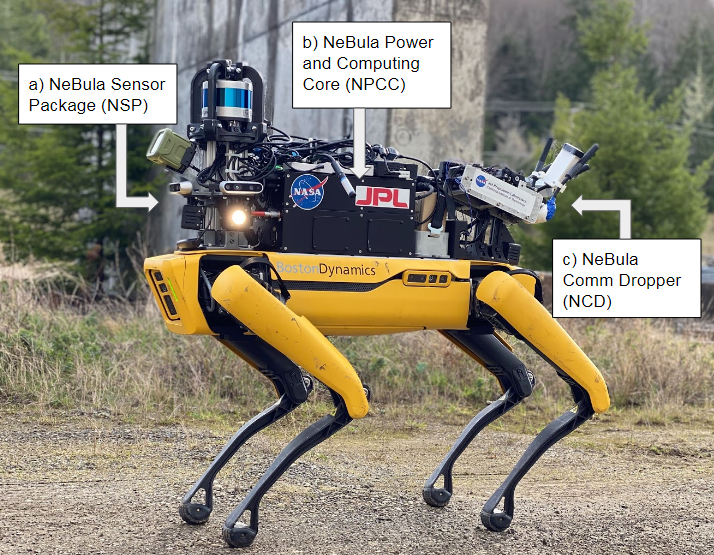
\includegraphics[width=0.5\textwidth]{spot_iros/graphics/spot_full_annotated_1.PNG}
  \caption{Spot in its full, NeBula powered form.}
  \label{fig:spot_full_nebula_form}
\end{figure}

%\begin{figure}[thpb]
 %  \centering
  %  \begin{subfigure}[t]{0.5\linewidth}
   %     \centering
    %    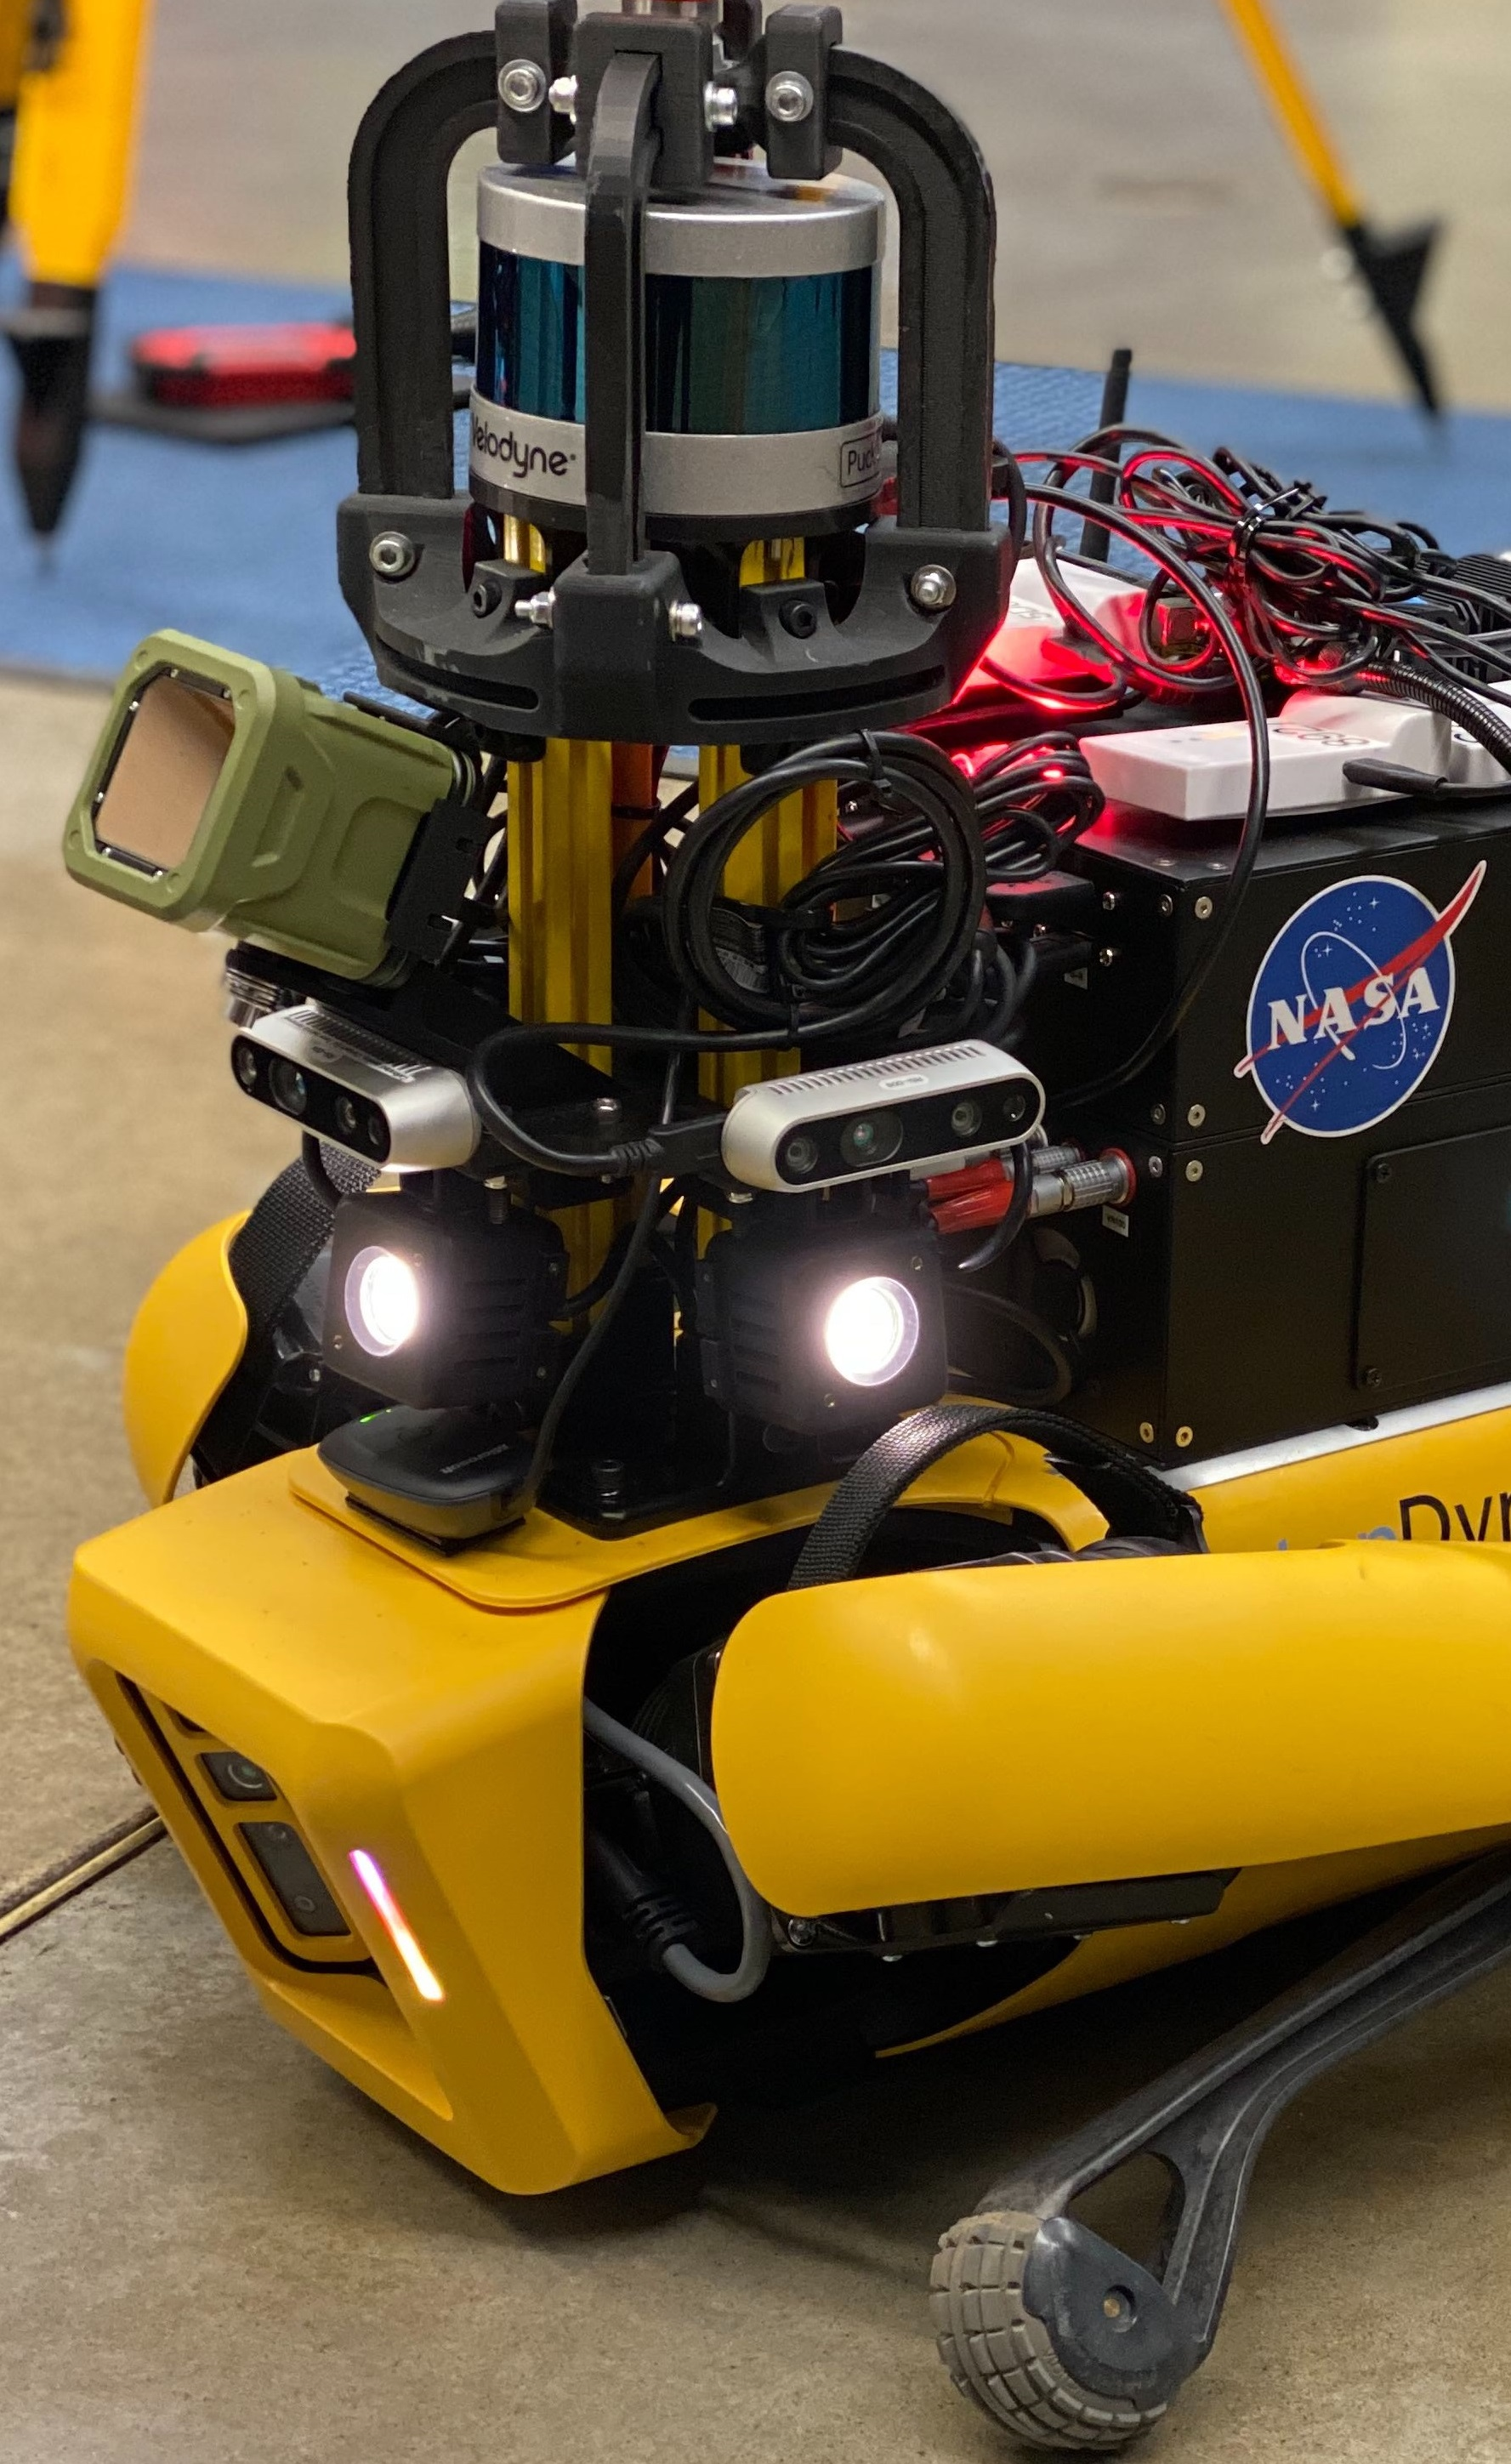
\includegraphics[width=\textwidth]{spot_iros/graphics/spot_sensor_package_NSP_2.jpg}
     %   \caption{Spot with Nebula Sensor Package Mounted}
      %  \label{fig:spot_payload_sens}
    %\end{subfigure}%
 %~
  %  \begin{subfigure}[t]{0.5\linewidth}
   %     \centering
    %    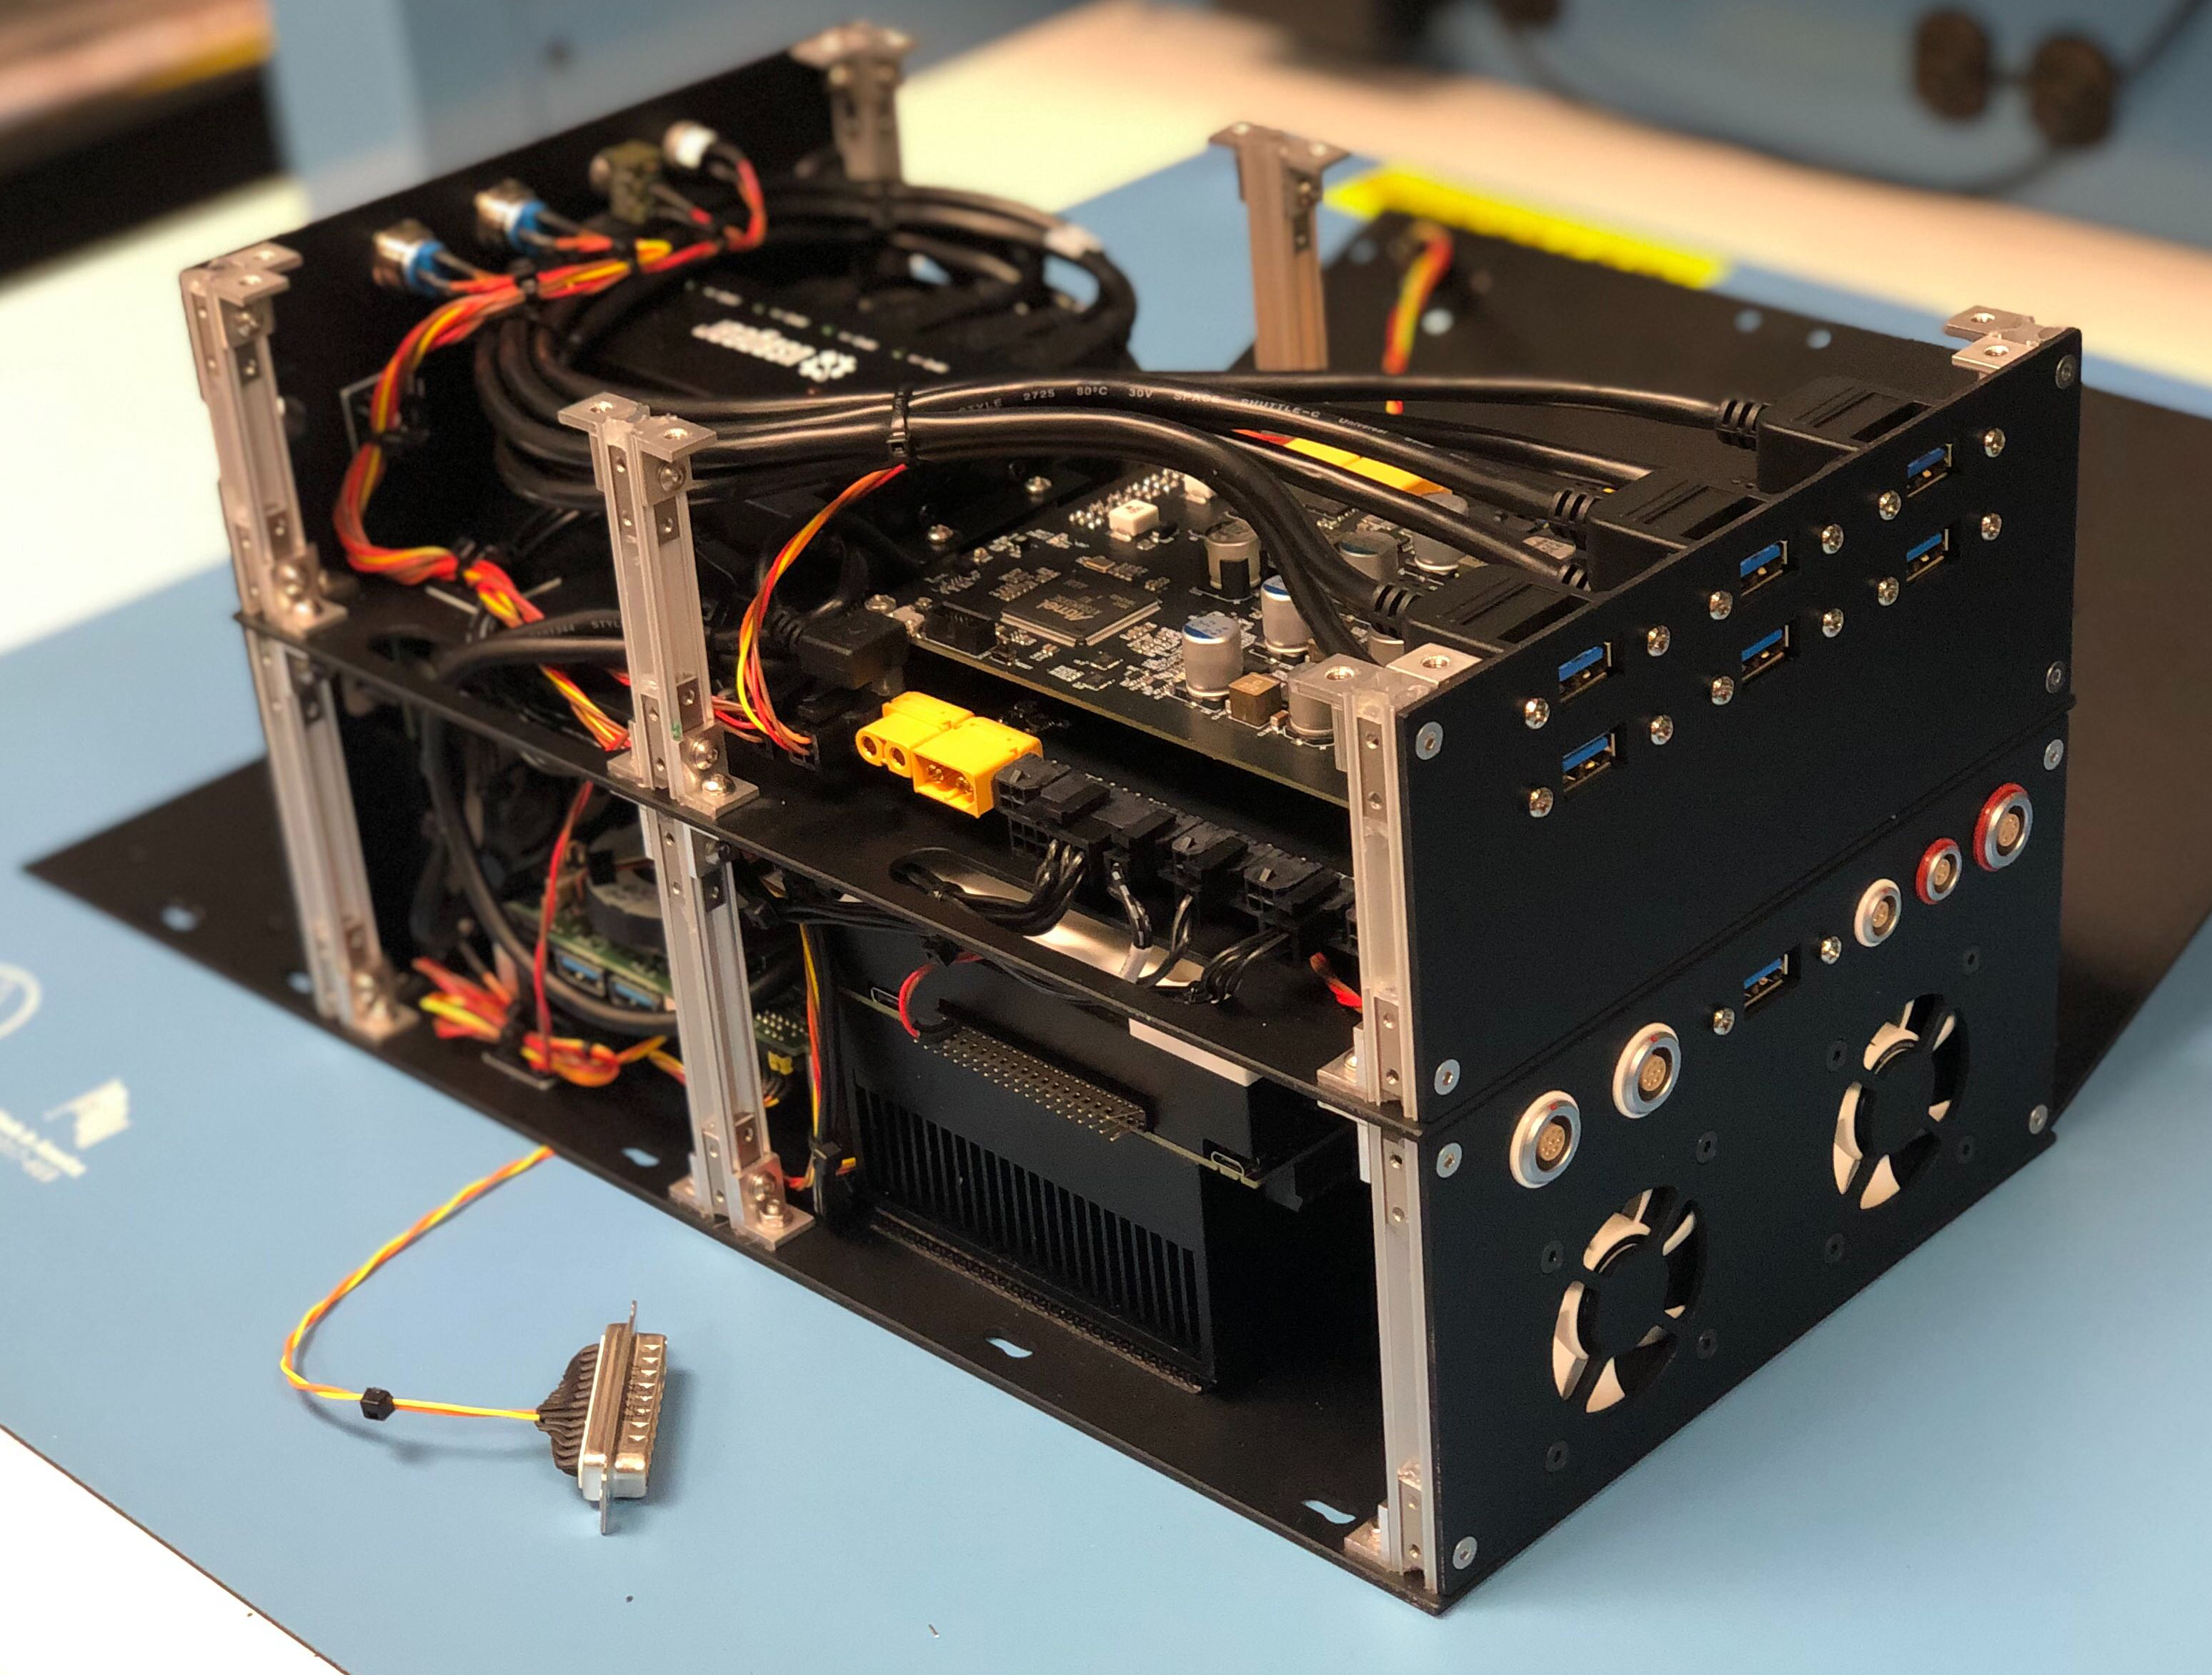
\includegraphics[width=\textwidth]{spot_iros/graphics/Spot_NPCC.jpg}
    %    \caption{Nebula Power and Computing Core with Covers Removed}
     %   \label{spot_payload_elec}
    %\end{subfigure}
    
%~
 %   \caption{NeBula Payload}
%\end{figure}

%\begin{figure}[h!]
%  \centering
%  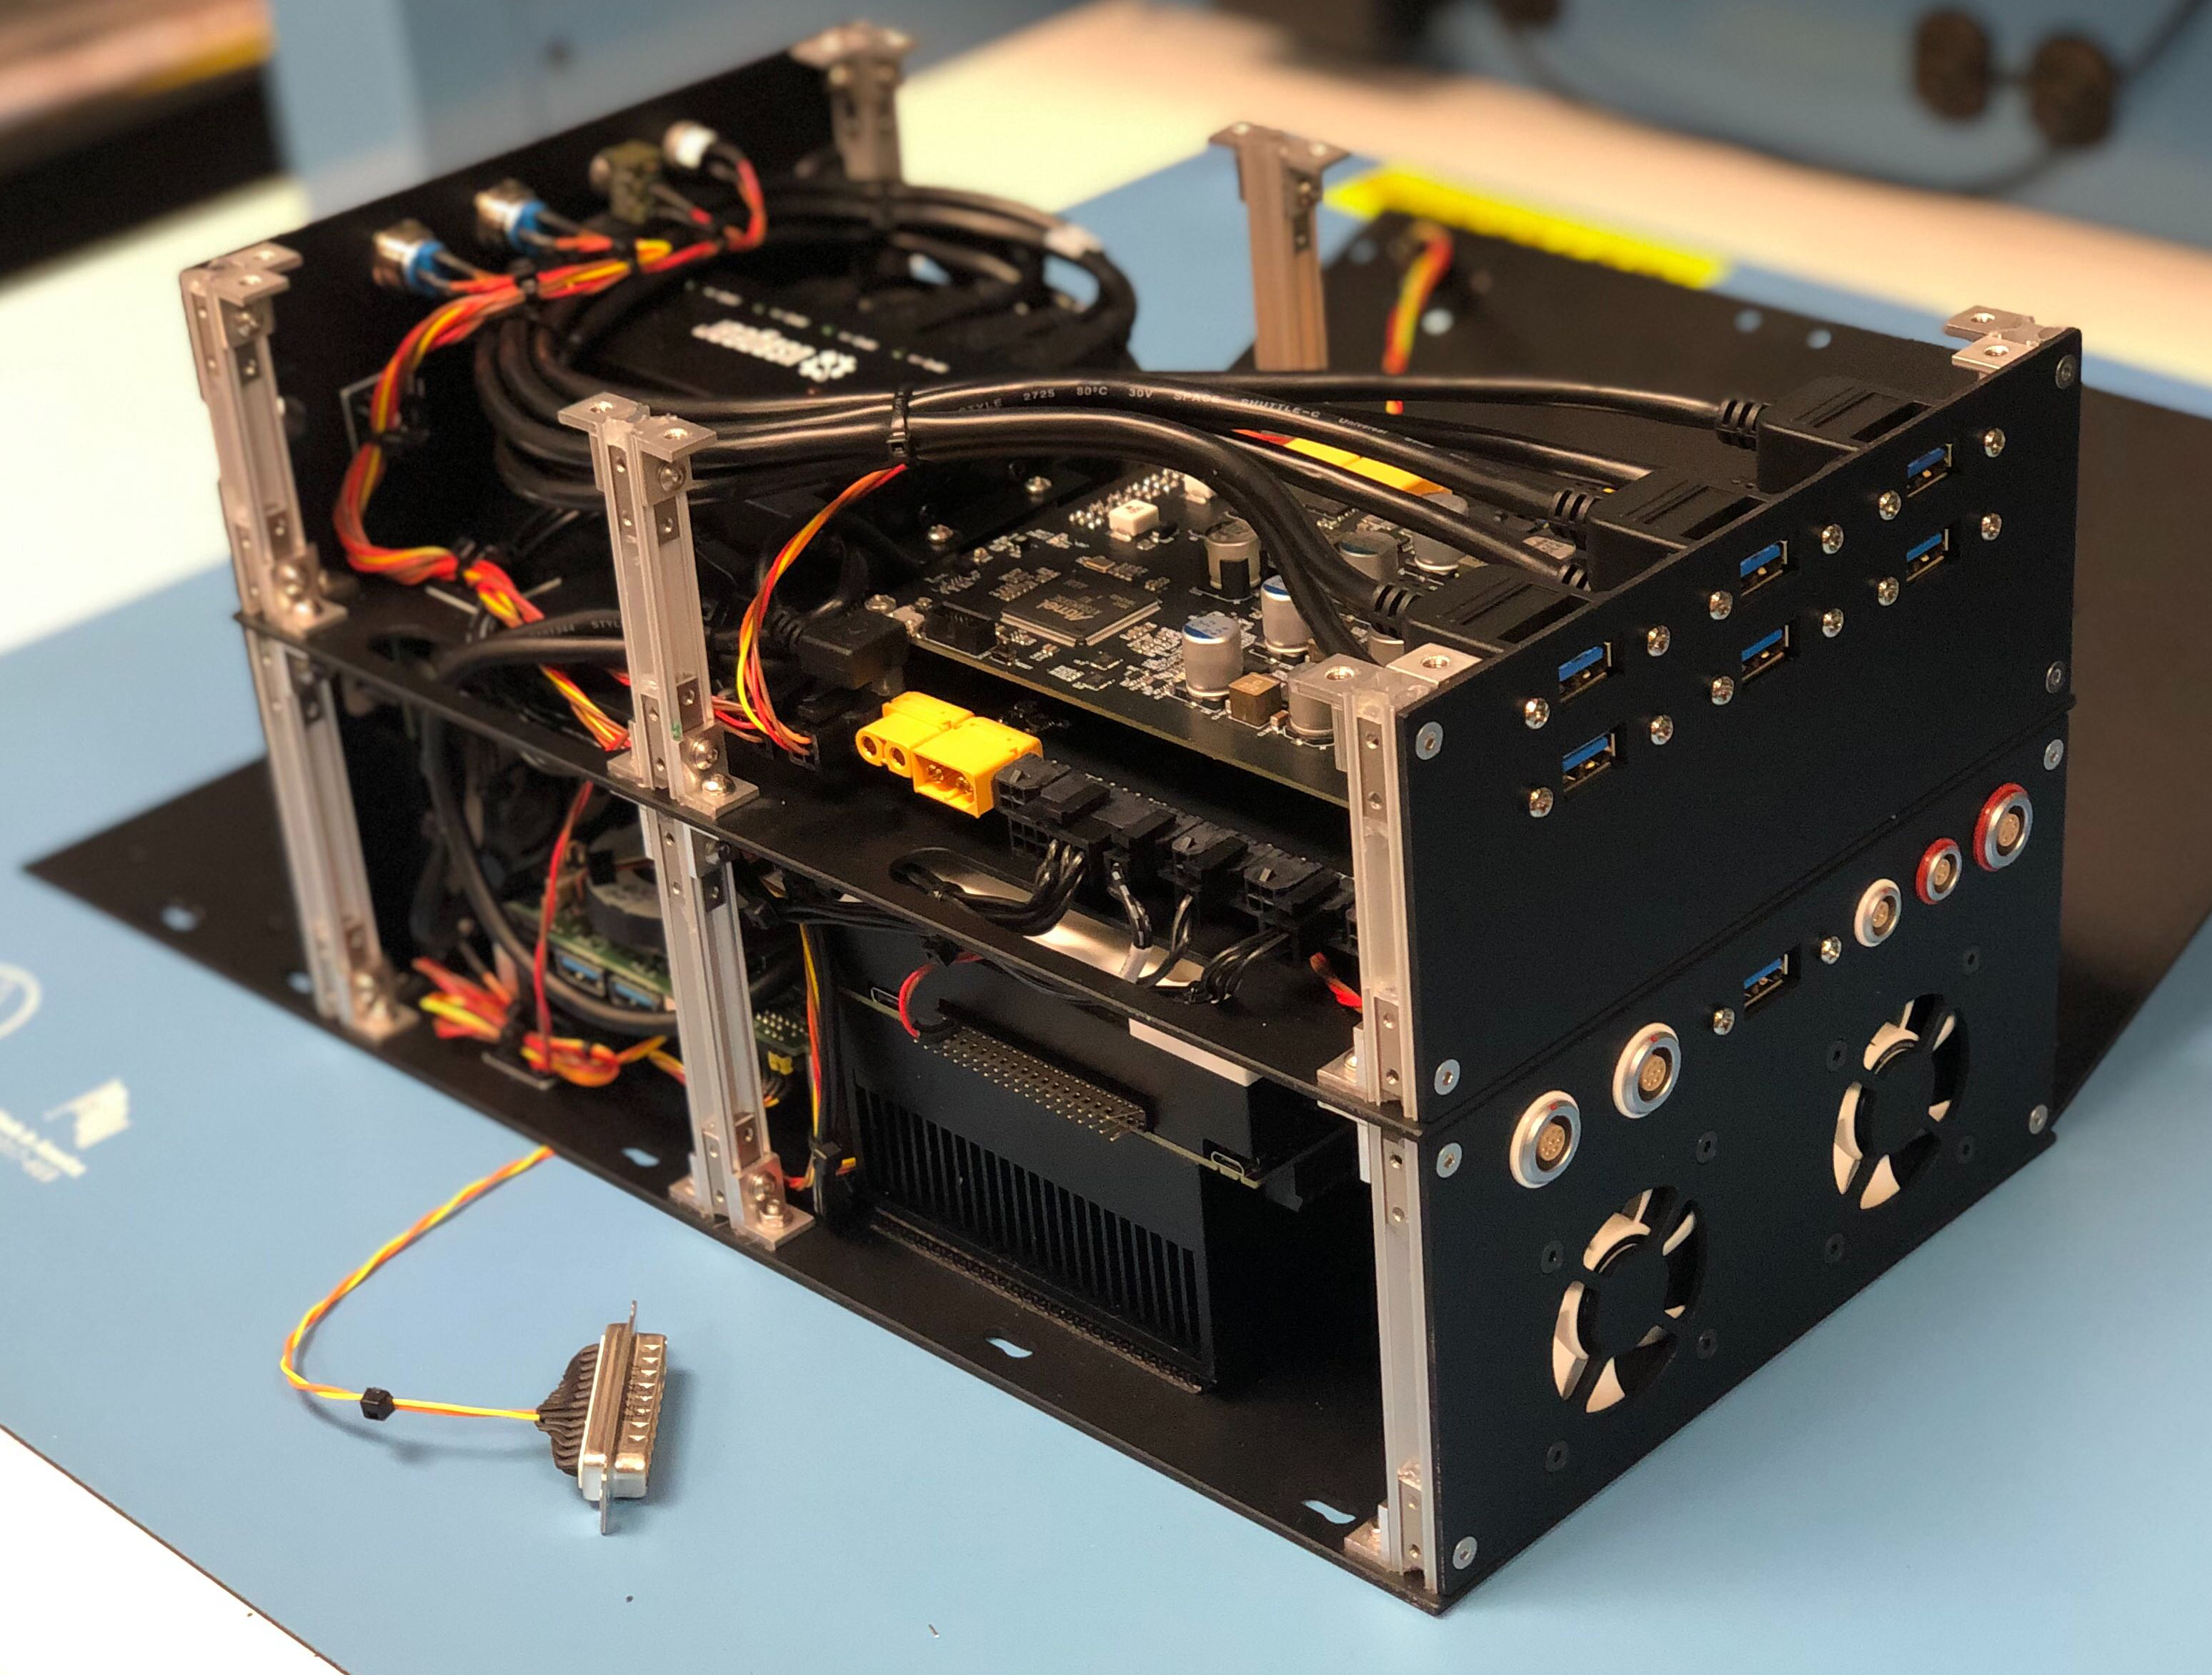
\includegraphics[width=0.3\textwidth]{spot_iros/graphics/Spot_NPCC.jpg}
%  \caption{Nebula Power and Computing Core with Covers Removed}
%  \label{fig:spot_payload}
%\end{figure}

% \inst{we dont need API discussion}
% \subsection{Spot Software Development API}
% \ph{Description of how program Spot through its accessible GRPC-based API and Python client library.}
% The Spot Software Development Kit enables your application to command poses and velocities, configure payloads, and access robot perception and payload data. Our Autonomy Software Development Kit, currently in Beta, will provide access to mapping, navigation, and mission editing. The API employs state-of-the-art security tools to keep your data secure.

% \ph{Robot State provided by the API and what we user}

% \ph{How to control the robot and what features are available}
% Locomotion parameter, allow obstacle avoidance, swing heights etc

% \ph{Conclude the capability of Spot and why we need NeBula to make Spot fully autonomous}

%%%%%%%%%%%%%%%%%%%%%%%%%%%%%%%%%%%%%%%%%%%%%%%%%
% \subsection{Software Interface to NeBula} % Nar5
% \inst{not very clear to me what this subsection is yet. Let's finish other parts and see if we need this}
% \ph{Overview of system integration}

% \ph{For system integration, we built the Spot driver to connect Spot API to ROS}

%\ph{Spot State}
% Robot state that we think its useful. KO, VO, Joint states, battery health

%\ph{Spot Mobility}
% Mobility setup that we think its useful: stair mode, selfright, friction coeff etc
% Stair climbing


% Spot system description will include:
% \begin{itemize}
%     \item System and locomotion system overview
%     \item Sensors description
%     \item Interfacing with Spot with API
%     \item Accessible States of the robot
%     \item Accessible locomotion, navigation feature adjustments and what we really care
%     \item Conclusion of the capability of Spot and why we need NeBula to have fully autonomous operation
% \end{itemize}



%%%%%%%%%%%%%%%%%%%%%%%%%%%%%%%%%%%%%%%%%%%
\section{NeBula Odometry on Legged Systems}\label{sec:state_estimation}
%%%%%%%%%%%%%%%%%%%%%%%%%%%%%%%%%%%%%%%%%%%
%\todo{Matteo - DONE}\ph{Challenges}
A reliable odometry source in perceptually-degraded settings is a challenge. The characteristics of the environment pose significant difficulties on various sensing modalities and strong platform vibration originated by mobility-stressing terrains introduces additional uncertainty on sensor measurements. Uneven and slippery areas make inertial sensing inaccurate while the material composition of the surface where the legged robot is walking on (e.g soft moquette, hard concrete) has strong impacts on the accuracy of kinematic-based odometry (KO). Darkness, or sudden excessive change in illumination, along with dust and occasional presence of fog and gas, pose significant issues in the camera domain, and potential visual aliasing phenomena in texture-less or texture-repetitive environments make feature-tracking problematic, decreasing the overall reliability of vision-based odometry (VO). Self-similar environments with repetitive geometry and lack of distinctive landmarks, makes scan-matching based methods ambiguous and prone to drift: moreover, active stereo cameras (including the ones on the Spot platform) have limited field of view and their high noise in long-range sensing render them inaccurate for the purpose. %All these challenges are in harsh contrast with the need of a reliable and accurate odometry source which is a key requirement in achieving precise robot localization to support a wide variety of applications, ranging from disaster response to the exploration of underground extraterrestrial worlds.

%\todo{matteo} \ph{Challenges}
%A reliable odometry in a perceptually-degraded setting is a challenge. Some elements of the course that contribute to sensing challenges are 1) self-similar terrains that provide a repetitive geometry confusing scan matching based methods, 2) variable lighting from full dark to lit that impose challenges to visible-light cameras, 3) platform vibration due to mobility-stressing terrains that create challenges for various sensing modalities, 4) limited field of view that renders depth cameras (including Spot's on-board depth cameras) unreliable where the long-range data is required for odometry, and 5) The material composition of the surface where the legged robot is walking on (e.g soft moquette, hard concrete) has a strong influence on the kinematic-based sensing.

%, and potential visual aliasing phenomena can degrade the generated VO in self-similar environments where poor, or self-repetitive texture make the feature tracking problem ambiguous and challenging. As KO would work better than VO in some cases, and VO better than KO in some others, this leads us to conclude that we can not therefore rely on these odometry sources as a SLAM front-end when exploring a wide range of different extreme environments.

%We analyze the performance of our SLAM system when feeding to the front-end point cloud data captured by the on board Realsense cameras. Fig.4 shows the front-end map constructed by Spot during the exploration of an indoor office: in a) the map produced by the front-end with pure point cloud odometry, in b) the map produced by the front-end with point cloud odometry where incremental transformations coming from VO are used to seed GICP during scan-to-scan registration. 

%As clearly visible, there is no chance of using Spot on board cameras to achieve accurate SLAM operation due to the high noise present in the far-field information of the point cloud data acquired from Realsense, that makes precise registration highly prone to errors, both in the scan-to-scan and in scan-to-submap stage. 

%\todo{matteo} \ph{High-level principles and requirements for the solutions}
%To address these challenges, NeBula relies on a multi-sensor solution to enable odometry in perceptually-degraded setting. Characterizing uncertainty associated and failure modes associated with each sensing modality, NeBula and fuses various sensing modalities in an uncertainty-aware manner. \inst{maybe draw a simple architcture diagram here (similar to HeRO).}

%\ph{High-level principles and requirements for the solution}


%, we realize SpotFrontend which is utilized as the front-end of a pose-graph solution to... 
%light-weight?

%At this point, we investigate on the other possibility of using as SLAM front-end the on board odometries natively provided by Boston Dynamics, namely KO and VO: from our tests, feeding KO or VO directly into LAMP back-end, can result in different and very unexpected effects that are highly susceptible to the environment type. 

%\ph{Overview} In this section we investigate on Simultaneous Localization And Mapping (SLAM) accuracy and robustness achievable with Spot onboard sensors when the robot is involved in the autonomous exploration of large-scale and perceptually-degraded extreme subterranean environments. We firstly break down the SLAM problem into its two main components, namely front-end and back-end and conclude that the on board sensors of Spot are not suitable to provide a reliable front-end module for robust SLAM operation. We then present a light-weight front-end solution that enables Spot to achieve accurate localization and mapping in such kind of scenarios by integrating the onboard Visual Odometry (VO) data feed with Lidar information. We provide experimental results showing that the proposed method consistently overcomes the available onboard localization accuracy, and we finally discuss the lessons learned.

\todo{Matteo} \ph{Proposed solution}
%To address these challenges, NeBula relies on a multi-sensor solution to enable accurate odometry generation in perceptually-degraded conditions via characterizing uncertainty and failure modes associated with each sensing modality. Here, we will go over the core part of this sensor fusion framework, where we fuse the kinematic odometry and visual odometry with Lidar information. The key idea is to use the incremental transformations coming from VO to seed the Generalized Iterative Closest Point (GICP) algorithm in the scan-to-scan registration stage: more specifically, we initialize GICP between the Lidar scan collected at the current time t and the Lidar scan collected at time t-1 with a rigid body transformation equal to the difference of VO pose at time t and VO pose at time t-1. As Boston Dynamics provides VO at 10 Hz, we use ROS Message Filters policies for waiting to have in the VO buffer data with a greater timestamp of the incoming Lidar message to be processed: this enables us to interpolate VO poses at Lidar timestamps and therefore obtain more accurate VO incremental transforms to be used as initial guess for GICP, which is a key requirement in achieving highly accurate odometry estimates from the front-end module. After the scan-to-scan stage is completed, a scan-to-submap matching refinement step is operated, where the latest scan is matched against a local submap [CIT. LAMP PAPER], and the overall final odometry estimate is delivered as output. 
In this section, we go over the core part of the above mentioned sensor fusion framework where we fuse a \emph{selected} external odometry source with Lidar information to enable accurate odometry generation in extreme environments. At first, multiple and heterogeneous odometries (e.g KO, VO, VIO, TIO) are feeded into an Odometry Multiplexer with Health Monitor and Switch On Failure Capability \cite{Santamaria-navarro2019} which outputs, at every time $k$, the data coming from the most relieable input realizing therefore a resilient and uncertainty-aware paradigm. Extending the work presented in \cite{Ebadi2020}, we feed the selected external odometry source into a front-end module that operates scan-to-scan and scan-to-submap matching in order to estimate the relative motion of the robot between consecutive Lidar acquisitions. The key idea is to use the incremental transformations coming from the external odometry source to seed the Generalized Iterative Closest Point (GICP) algorithm in the scan-to-scan registration stage: more specifically, we initialize GICP between the Lidar scan collected at the current time $k$ and the Lidar scan collected at time $k-1$ with a rigid body transformation equal to the difference of the external odometry pose at time $k$ and the external odometry pose at time $k-1$. Since the external odometry source could arrive at unexpected rates, we use ROS Message Filters policies for waiting to have in the external odometry buffer, data that has a greater timestamp of the incoming Lidar message to be processed: this enables us to interpolate external odometry poses at Lidar timestamps and therefore obtain more accurate external odometry incremental transforms to be used as initial guess for GICP, which is a key requirement in achieving highly accurate odometry estimates in the front-end module. To further enhance the accuracy of the scan-to-scan estimate, we also use a scan-to-submap matching step, where the latest scan is matched against a local submap: after this step is completed, the final odometry estimate is delivered as output. 

\begin{align}
    T^*_k &= \arg\min_{T_k} d(T_k PC_k, M_k; T^*_0) \\
    T^*_0 &= \arg\min_{T'_k} d(T'_k PC_k, PC_{k-1}; T'_0)\\
    T'_0 &= KVO(z_k, z_{k-1})    
\end{align}

\begin{figure}[thpb]
  \centering
  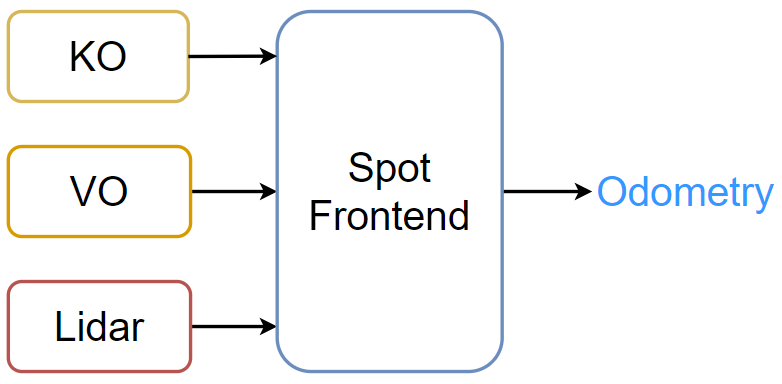
\includegraphics[width=0.35\textwidth]{spot_iros/graphics/spot_spot_frontend.PNG}
  \caption{Multi-sensor fusion in Spot Frontend}
  \label{fig:spot_frontend}
\end{figure}

\todo{Matteo - DOING} \ph{Global mapping}
The odometry produced by the proposed front-end is then fed into a pose-graph

Our 3D SLAM system \cite{Ebadi2020}, referred to as LAMP (large-scale autonomous mapping and positioning) is comprised of two fundamental components: a front-end and a back-end. 

The odometry produced by the proposed method is then fed into a pose-graph as the front-end pose-to-pose constraints: in the back-end we solve a Pose Graph Optimization (PGO) and Incremental Consistency Measurement (ICM) for global localization and detecting Loop Closures during traverse and optimize the graph accordingly. 

%%%%%%%%%%%%%%%%%%%%%%%%%%%%%%%%%%%%%%%%%%%
\section{Local Planning}\label{sec:local_planning}
%This section describes our approach to build a bigger environment map and it's use for local planning.

\ph{Traversability Analysis}
Assessing traversability and risk is prerequisite to autonomous navigation in extreme environments.  These traversability challenges, which have to be accounted for by a local planner, include high slopes, obstacles, holes, comm nodes dropped by the robot or sensor blind spots.  In order to find a balance between efficient traversal and low risk to the platform, we construct a measure of accumulative risk for a given path through the environment.  Let $g=(m^1,\cdots,m^n)$ be a grid of $n=n_l\times n_w$ cells with length $n_l$ and width $n_w$, and let each $m^i\in[0,1]$ represent the probability that the robot safely traverses through the cell.  Let $\pi=\{i_t\}_{t=0}^T$ be a sequence which defines a connected path through the grid, and define the solution space $\Pi$ as the set of connected paths through the grid which connects the current robot position with the goal.  Then we define the total accumulated risk of the path $\pi\in\Pi$ as 
\begin{align}
 \mathcal{R}^{\pi}=1-\prod_{t=0}^Tm^{i_t}
\end{align}
which is the probability that the robot fails to safely traverse the path $\pi$.  


\ph{Sources of Risk} We combine multiple layers of grids which encode different types of risk.  Assuming mutual exclusivity between each risk type, the total risk in each grid cell is simply the product of the individual risks of each layer.  We consider the following sources of risk:
\begin{itemize}
    \item Obstacles (Walls, Rubble, etc.)
    \item Steep Slopes
    \item Negative Obstacles
    \item Sensor Blind Spots
    \item Mission Items (comm nodes, other robots, etc.)
\end{itemize}
To identify these sources of risk, we perform traversability analysis on a local map generated from KO/VO odometry and sensor measurements (depth camera, LiDAR).  We fit local ground planes on the map to identify traversable ground regions.  Ground planes which have too high of a slope are identified as "Steep Slope" regions.  Points on the map which are above or below the ground plane which are higher than the ground clearance of the robot are marked as "Obstacles".  Negative obstacles are identified by gaps in the map (where no sensor measurements are available).  Sensor blind spots contribute a non-lethal risk and are identified by the respective sensor models.  Finally, we add mission-specific items to the risk map (to avoid dropped comm nodes, other robots, etc.)  

%Accurate risk assessment is contingent upon good localization/odometry.  When odometry fails we want our assessment of risk to remain conservative in such a way as to keep the vehicle safe at all times.  Therefore we rely on a multi-resolution approach for assessing risk.  We asses risk on a local scale (2m radius) by relying on wide-field of view sensor data with a short temporal window.  This approach relies on a short history of KO/VO odometry, which tends to have low drift at these timescales.  For areas outside this small radius (2m-10m), we rely on temporally fused sensor data using our LiDAR payload, since this sensor has much longer range and higher accuracy at these scales.  We combine these two layers to achieve both long-range mapping for efficient planning, along with high-fidelity mapping at short ranges to ensure the safety of the platform.

\ph{Solver}
We search for the minimum risk path using A*:
\begin{align}
    \pi^* = \arg\min_{\pi\in\Pi}\mathcal{R}^{\pi}(g)
    \label{deterministic_plan}
\end{align}
Having found the minimum risk path, we then send a carrot waypoint 1m along this path to the BD internal planner.  Because the internal BD sensor configuration has a limited field of view, it is much safer and more effective for the robot to prefer moving in the forward direction, where sensor coverage is better.  In general, within the NeBula framework, we formalize this notion with a perception-aware planner.

\ph{Uncertainty-aware Representation}
We model each cell $m^i$ as a random variable, where $\hat{m}^i$ and $\sigma^{m^i}$ denote its mean and variance. The "information" about $m^i$ is captured in the $\sigma^i$, where fully unknown and fully known cells have the highest and lowest $\sigma^i$ values, respectively.  By explicitly capturing the learned information about each cell $m^i$, we can treat all the cells (known, unknown, partially-known) in a unified manner. 

\ph{Uncertainty-aware map prediction}
This representation allows us to incorporate perceptual capabilities (hence the name "perceptual" in NeBula) into the planning. Given the sensors available on the robot and their configuration and noise characteristics, we can derive models that predict the evolution of $\sigma^i$ based on a sensor configuration and most likely measurements along a given trajectory $\pi$. 
\begin{align}
 \sigma^i_k = prediction( \sigma^i_0, z_{0:k}(\pi) )
\end{align}
where the measurements $z_0,\cdots,z_k$ are predicted at each of the first $k$ timesteps along the path $\pi$.
This becomes increasingly important when the sensor configuration is highly asymmetric on a robot, which is the case for Spot as it has blind spots and areas where sensory measurement noise is considerably higher than other areas.  We denote the predicted map $k$ time steps in the future along the trajectory $\pi$ by 
\begin{align}
 g_k = \{p(m|m^1_k,\sigma^1_k),\cdots,p(m|m^n_k,\sigma^n_k)\}   
\end{align}
where $p(m|m^i_k,\sigma^i_k)$ is the probability distribution of $m^i$ parameterized by $m^i_k$ and $\sigma^i_k$.
As a result, we define a risk measure that takes perceptual capabilities and uncertainties into account when planning trajectories, by minimizing accordingly:
\begin{align}
 \mathcal{R}_k^{\pi}=1-\prod_{t=0}^Tp(m|m_k^{i_t},\sigma_k^{i_t}),~~~
    \pi^* = \arg\min_{\pi\in\Pi}\mathbb{E}[\mathcal{R}_k^{\pi}(g_k)]
\end{align}
Efficient methods for computing predicted risk uncertainty over a 2-D grid for a given sensor model have been considered in \todo{CITE}.

\ph{Specific example Necessity of perception aware planing in Spot}
Although a key feature of NeBula is in planning perception-aware paths, in the case of integration of NeBula with Spot, we found that a simple heuristic sufficed to approximate the optimal solution $\pi^*$.  This heuristic was to solve for deterministic A* paths (Equation \ref{deterministic_plan}) and then to give a desired location and orientation to Spot as a waypoint along this path.  The orientation was simply the relative heading between the current robot position and the waypoint itself.  This results in a behavior where the robot orients itself forward as it walks whenever possible.  We found this heuristic to be sufficient in practice since Spot is a holonomic robot and can orient itself in any direction as it moves.  Furthermore, the sensor coverage from Spot's internal cameras is Figure \ref{bd_costmap} shows an example costmap Future work will involve bringing the more advanced uncertainty-aware planning from the NeBula framework into Spot. 

\begin{figure}[thpb]
   \centering
    \begin{subfigure}{0.5\linewidth}
        \centering
        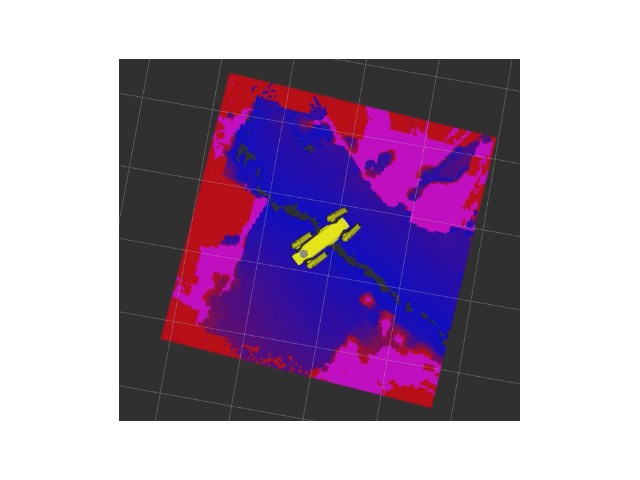
\includegraphics[trim={4cm 3cm 4cm 3.5cm},clip, width=\linewidth]{spot_iros/graphics/costmap_bd2.png}
    \end{subfigure}%
    ~
    \begin{subfigure}{0.5\linewidth}
        \centering
        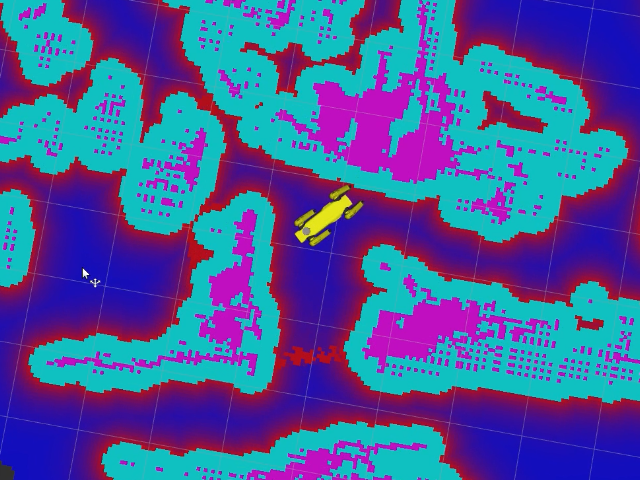
\includegraphics[trim={1cm 1cm 1cm 1cm},clip, width=\linewidth]{spot_iros/graphics/costmap_bd2_embedded.png}
    \end{subfigure}
    \label{bd_costmap}
    \caption{Left:  Risk map generated from BD onboard cameras, pink lethal, red high-risk but non lethal, and blue low risk.  Right:  BD risk map layer combined with LiDAR based risk map showing larger range of obstacles.}
\end{figure}

% \begin{itemize} % For Mission Autonomy(Behavstmap) -> iours, IRM) probably we just gonna cite Scott and Kyon aero paper. 
%         \item Traversability (settling, collision check, slope check, negative obstacles,..) (David?)
%     \item Local Planning (our traversability/local planner complements BD's internal one. We have long range LiDAR, bigger costmaps and detect negative obstacles. In the local planner, we can encourage forward motion in order to avoid walking into the robot's blind spot and increasing the chance of seeing artifacts with the forward facing sensors)
% \end{itemize}

%%%%%%%%%%%%%%%%%%%%%%%%%%%%%%%%%%%%%%%%%%%
\section{Mission planning}\label{sec:mission_planning}
%\inst{not clear if we need this section}
\todo{Scott-Kyon-FadNik} \ph{Mission and its challenges} In the SubT Challenge, robots are expected to rapidly map, navigate, and search unknown underground environments, and report back to the human supervisor at the base station. Particularly, the Urban Circuit posed many challenges to the autonomous robot teams, including complex topology (e.g., multiple stories, dead-ends, various types of junctions, narrow corridors to big open spaces), mobility challenges (e.g., stairs, vertical shafts), and intermittent communications to the base and the other robots due to non-line-of-sight structures. Robots are programmed to autonomously detect and explore the new frontiers, as well as sharing the distinctive environmental elements such as stairs and major forks back to the base station. If the robots lose communications while pushing the frontier forward, two droppable communication nodes are deployed to maintain contact.

\todo{Scott-Amanda-Sung} \ph{Behaviours and Modes}
Hence, there are high-level bahviors in the mission planning layer. We denote the behavior library as
\begin{align}
    \mathcal{B} = \{B^1,\cdots,B^n \}
\end{align}
The role of mission planner is to generate a sequence of behaviors
\begin{align}
    (B_0,B_1,\cdots,B_T) = \arg\min MissionRisk(\mathcal{B})
\end{align}
A given behavior $B^i$ is executed by visiting a set of anchor points in the information space as explained in the next paragraph. 

%========= \inst{Ali has read up to this point}

\todo{Sung-Amanda-David} \ph{IRM} To quantify the above-mentioned mission risk, we first create a sparse graph structure ($G$) to capture the connectivity of the free space in a big complex environment:
\begin{align}
    G = (V, E)
\end{align}
We refer to this graph as the IRM (information roadmap) as its nodes ($V$) and edges ($E$) are enriched by various environmental and robot-related properties. As an example, in the Urban Circuit, a node at the entrance of a staircase is marked with a special attribute which indicates that a high level of traversability, unique to Spot, is required to plan paths through this node. 

IRM nodes are categorized as either breadcrumbs ($\beta$), frontiers ($f$), or the home base ($h$) where the mission is initiated. 
\begin{align}
    V = (f, \beta, h)
\end{align}
Pose graph-fixed breadcrumb nodes trace the history of the robot's motions and, hence, indicate both known areas and traversable paths via breadcrumb edge connections. Frontier nodes are located at the boundary between unexplored and known space, and are connected to breadcrumb nodes though collision-free edges. Furthermore, since robots share their pose graph with one another, frontier nodes are never placed in already explored areas.  
%Also, frontier nodes and their edge connections on the IRM encode where the unexplored regions are, how significant they are for the global coverage, and how to traverse to them in this multi-level environment.
%The global planning module provides services to maintain and query the IRM, such as adding/pruning frontier nodes. Behaviors can query the global planner for the shortest path to frontiers, closest stairs, and the base station. Additionally, the planner is responsible for ensuring that the locations of the IRM nodes remains consistent after a pose-graph relaxation from the global localization module.  

% \begin{align}
%     E = (T, D, ...)
% \end{align}

\todo{Amanda-David-Sung} \ph{Planning} 
The objective of the global planning module is to assign frontiers as terminal goals as to maximize global coverage of the environment by multiple robots, including Spots, for the allotted time. Frontier goals are assigned to the robot according to either a local or global selection approach. 
\subsection{Local Frontier Selection}
Given the robot's current pose ($x_k$), we select a frontier goal ($f_g$) with minimum bearing (i.e. planar angle between robot's forward direction and frontier location), subject to traversability and bearing constraints:
\begin{align}
    J^{local}(V, E, x_k) &= \theta_{bearing}(x_k, f) 
\end{align}
\begin{align}
    f_g &= \arg\min_{f\in V} J^{local}(V, E, x_k)\\
    ~s.t.,~~~ & P_{travs}(x_k, f) > \gamma \nonumber \\
    % & f \in Disc(x_k, r)\\ NOTE we choose this range so we can make a judgement about traversability, so prob not necessary to make it a separate constraint
    & \theta_{bearing}(x_k, f) < \zeta \nonumber
\end{align}
Note that for the local frontier selection, the frontiers in the direction of robot's current heading are preferred in order to minimize velocity changes during traversal. This scheme is particularly helpful for Spot so that it can walk continuously at higher speed and minimize turning motions which may cause risky foot placements at the blind spots (at the rear-left and -right) of the robot.
\subsection{Global Frontier Selection}
Global frontier selection is initiated if no frontier exists satisfying local selection constraints. Frontiers ($f$) in the IRM ($G$) are clustered according to the minimum number of edges connecting any two sets of observations through a hierarchical agglomerative clustering strategy. 

\todo{Not sure how to write this cluster eqn}
\begin{align}
    % cluster(f) = \{ f' | d(f', f) < n_{E} \}\in\mathcal{C}
    C(f) = \{ f' | dist(f', f) < n_{E} \}\in\mathcal{C} 
\end{align}
Since cluster size is indicative of an unexplored region's expanse, we use it to predict expected information gain, or the utility of traversing to a frontier in that cluster ($C(f)$). For a given cluster, the minimum number of edges between the robot's current position and that cluster is the cost of traversal. We select a frontier goal ($f_g$) closest to the centroid of the cluster ($C_g(f)$) which maximizes our cost-utility function:
\begin{align}
    J^{global}(V, E, x_k) = w_{d} \cdot \frac{1}{dist(x_k, f)} + w_{s} \cdot |C(f)|
\end{align}
\begin{align}
    f^{*} &= \arg\max_{C\in \mathcal{C}} J^{global}(V, E, x_k), \quad  f^* \in C_g(f)\\
    % ~s.t.,~~~ & dist(x_k, C) < \gamma' \nonumber \\
    f_g &= \arg\min_{f\in C_g(f)} dist(f, centroid(C_g(f)))
\end{align}
A robot travels to a global frontier goal by backtracking and planning paths along its breadcrumbs.
% Since the robots share their explored regions with each other, the global planner can automatically deploy them to different sectors of the environment. 




% \begin{align}
%     J(V, E; x_k) = dAng(f, x_k)
% \end{align}

% \begin{align}
%     nextWyapoint &= \arg\min_{f\in V} J(V, E)\\
%     ~s.t.,~~~ & P(f, x_k) > \gamma \\
%     & f \in Disc(x_k, r)\\
%     & dAng(f, x_k) < \zeta
% \end{align}
% \begin{align}
%     cluster(f) = \{ f' | d(f', f) < r \}\in\mathcal{C}
% \end{align}


% \begin{align}
%     J^{global}(V, E; x_k) = w_s |Cluster(f)| + w_d degree(f)
% \end{align}

% \begin{align}
%     C^s &= \arg\max_{c\in \mathcal{C}} J^{global}(V, E)\\
%     ~s.t.,~~~ & d(C, f) < \gamma' \\
% \end{align}

% \begin{align}
%     f^* &= centroid(C^s)
% \end{align}


\begin{figure}[thpb]
  \centering
  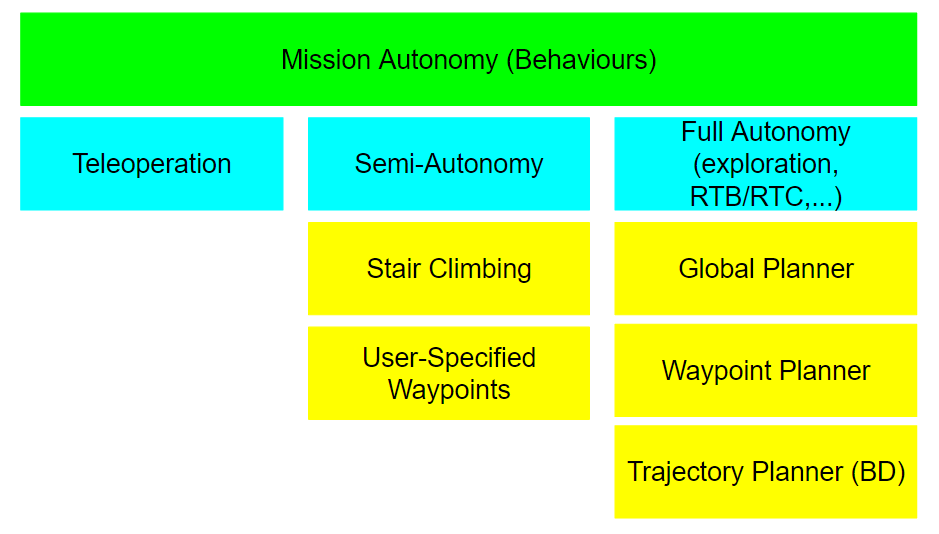
\includegraphics[width=0.40\textwidth]{spot_iros/graphics/spot_planning.PNG}
  \caption{\inst{not sure if we need this} Planner Architecture on Spot. TODO@Nikhilesh: Make cleaner graphic}
  \label{figurelabel}
\end{figure}

% Then, we need to discuss how traversability and risk values (from the previous section) appear on IRM edges... \inst{since we are not doing this yet, this might need some coding or we can remove this section}... similarly, we should show how stairs semantics appear on teh IRM... similarly, we can discuss when the robot calls operator for help (it shoudl be the "result" of planning. for example, when the planning returns a plan which has a risk beyond 70 percent). The output of planning could be from a activity library (e.g., explore, rtb, rtc, teleop, stair climbing,...). This set (activity library) needs to be defined mathematically and the plannign probelm shoudl be formulated as a optimization over this activity library space.



%%%%%%%%%%%%%%%%%%%%%%%%%%%%%%%%%%%%%%%%%%%
\section{Experimental Results}\label{sec:experiments}
%%%%%%%%%%%%%%%%%%%%%%%%%%%%%%%%%%%%%%%%%%%

The NeBula autonomy framework is implemented on two Spot robots and tested in various multi-story buildings. In particular, the NeBula-powered Spots were deployed onto the unfinished power plant in the Satsop Business Park during the DARPA SubT Challenge Urban Circuit in February 2020. Two Spots were able to explore multi-level environments and report back accurate artifact locations to the human supervisor at the base station.

\ph{Odometry Estimation}
To demonstrate the performance of the multi-modality odometry on a legged system, we evaluate and compare the localization accuracy using individual sensing channels with the proposed uncertainty-aware multi-sensor approach in perceptually-degraded environments. 

Fig. \ref{spot_eagle_rock} depicts the results of the proposed method on Eagle Rock data (where KO in LAMP bad, VO in LAMP good), while in Fig. \ref{spot_indoor_office} results of the proposed method in 198/161 data (where KO in LAMP good, VO in LAMP bad). 

%of the proposed method. As it can be seen, feeding LAMP with odometry estimates computed by Spot Frontend consistently overcomes the performance achievable with native Boston Dynamics provided odometries (KO/VO). 

We therefore conclude that we propose a more robust and accurate perception pipeline to enable high-fidelity robot localization and mapping in perceptually-degraded environments. Moreover, the proposed front-end is computationally light-weight and therefore accounts for the limited computational capability of the on board processing unit.

The proposed solution has been employed as front-end for the two Spot robots of CoSTAR Team during the exploration of a dismissed multi-level power plant in Elma, WA for the Urban Circuit of DARPA SubT Challenge where CoSTAR Team won the first place.

\begin{figure}[thpb]
  \centering
  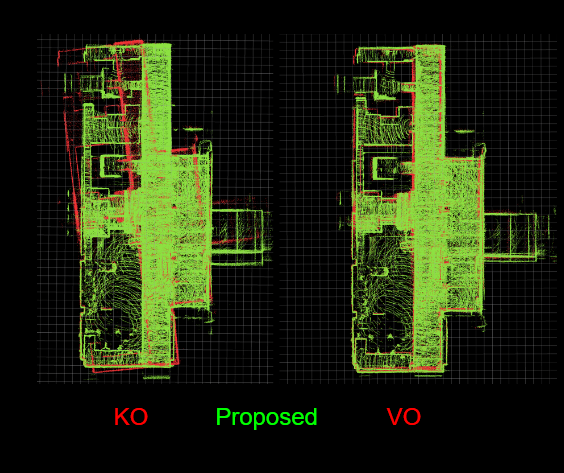
\includegraphics[width=0.47\textwidth]{spot_iros/graphics/spot_eagle_rock.PNG}
  \caption{Spot exploration of Eagle Rock: proposed method in green against a) LAMP KO and b) LAMP VO}
  \label{spot_eagle_rock}
\end{figure}

\begin{figure}[thpb]
  \centering
  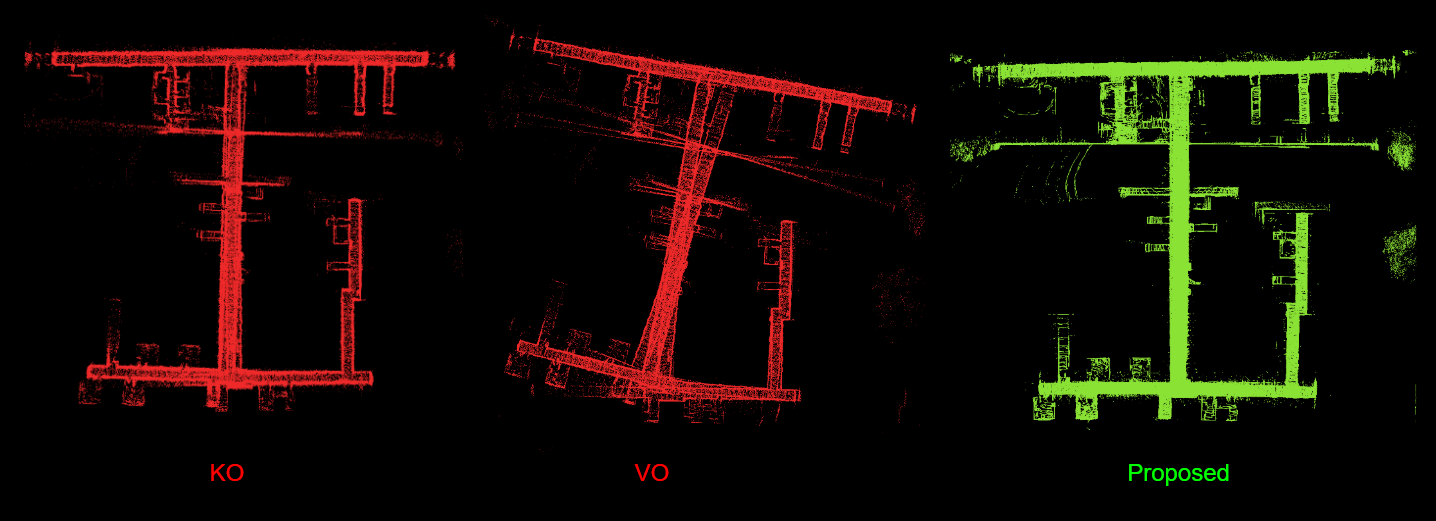
\includegraphics[width=0.47\textwidth]{spot_iros/graphics/spot_198_office.PNG}
  \caption{Spot exploration of an indoor office: a) LAMP KO b) LAMP VO c) Proposed}
  \label{spot_indoor_office}
\end{figure}

%%%%%%%%%%%%%%%%%%%%%%%%%%%%%%%%%%%%%%%%%%%
\subsection{Planning and Autonomous Exploration}
%%%%%%%%%%%%%%%%%%%%%%%%%%%%%%%%%%%%%%%%%%%
\textbf{Coverage Planner}
The exploration planner presented in Section \ref{sec:mission_planning} combined with the local planner presented in Section \ref{sec:local_planning} succesfully enabled two Spots to autonomously explore and map the underground environment of an abandoned nuclear power plant.

Figure ??? shows the map built and area explored by one of the Spots.
The Spot travelled ??? m in ??? min.

\begin{figure}[thpb]
  \centering
  \includegraphics[width=0.47\textwidth]{example-image-a}
  \caption{Area covered by exploration planner (topdown view)}
  \label{fig:exploration_planner_topview}
\end{figure}

\textbf{Multi--Level}
The fully autonomous exploration behaviour, combined with the semi--autonomous stair climbing capability, enabled the spots to explore the testing facility on multiple levels.
Figure ??? shows the reconstructed map from a multi--level exploration mission.

\begin{figure}[thpb]
  \centering
  \includegraphics[width=0.47\textwidth]{example-image-a}
  \caption{Exploration on Multiple Levels.}
  \label{fig:exploration_planner_multilevel}
\end{figure}

\textbf{Traversability}
The NeBula traversability analysis creates costmaps in the size of 20x20m, due to the usage of long--range sensors such as LiDARs, combined with spatial fusion.
This is crucial for bridging the gap between the Spot's internal planner, which only keeps a robot--centric environment map in the size of 4x4m, and the goals given by the global planner, which can be up to 10 m away from the robot's current position.

\begin{figure}[thpb]
   \centering
    \begin{subfigure}[t]{0.5\linewidth}
        \centering
        \includegraphics[height=1in]{example-image-a}
        \caption{Detecting Positive Obstacles}
        \label{fig:trav_costmap_pos_obs_wall}
    \end{subfigure}%
    ~ 
    \begin{subfigure}[t]{0.5\linewidth}
        \centering
        \includegraphics[height=1in]{example-image-b}
        \caption{Detecting Negative Obstacles (down stairs)}
        \label{fig:trav_costmap_neg_obs_stairs}
    \end{subfigure}
        \begin{subfigure}[t]{0.5\linewidth}
        \centering
        \includegraphics[height=1in]{example-image-a}
        \caption{Avoiding dropped comm nodes}
        \label{fig:trav_costmap_comm_nodes}
    \end{subfigure}%
    ~ 
        \begin{subfigure}[t]{0.5\linewidth}
        \centering
        \includegraphics[height=1in]{example-image-a}
        \caption{Avoiding Sensor Blind Spots}
        \label{trav_costmapb_bd_blindspot}
    \end{subfigure}%
    \caption{Traversability Costmaps}
\end{figure}

\textbf{Local Planning}
Complementing the internal planner, by using a custom local planner with a bigger horizon, helped avoiding suboptimal paths and avoid obstacles that could not be seen by the Spot's internal mapper, such as negative obstacles, obstacles far away.
\begin{figure}[thpb]
  \centering
  \includegraphics[width=0.47\textwidth]{example-image-a}
  \caption{Long--Range Costmap + Dijkstrapath + Waypoint}
  \label{fig:local_planner}
\end{figure}

\begin{figure}[thpb]
  \centering
  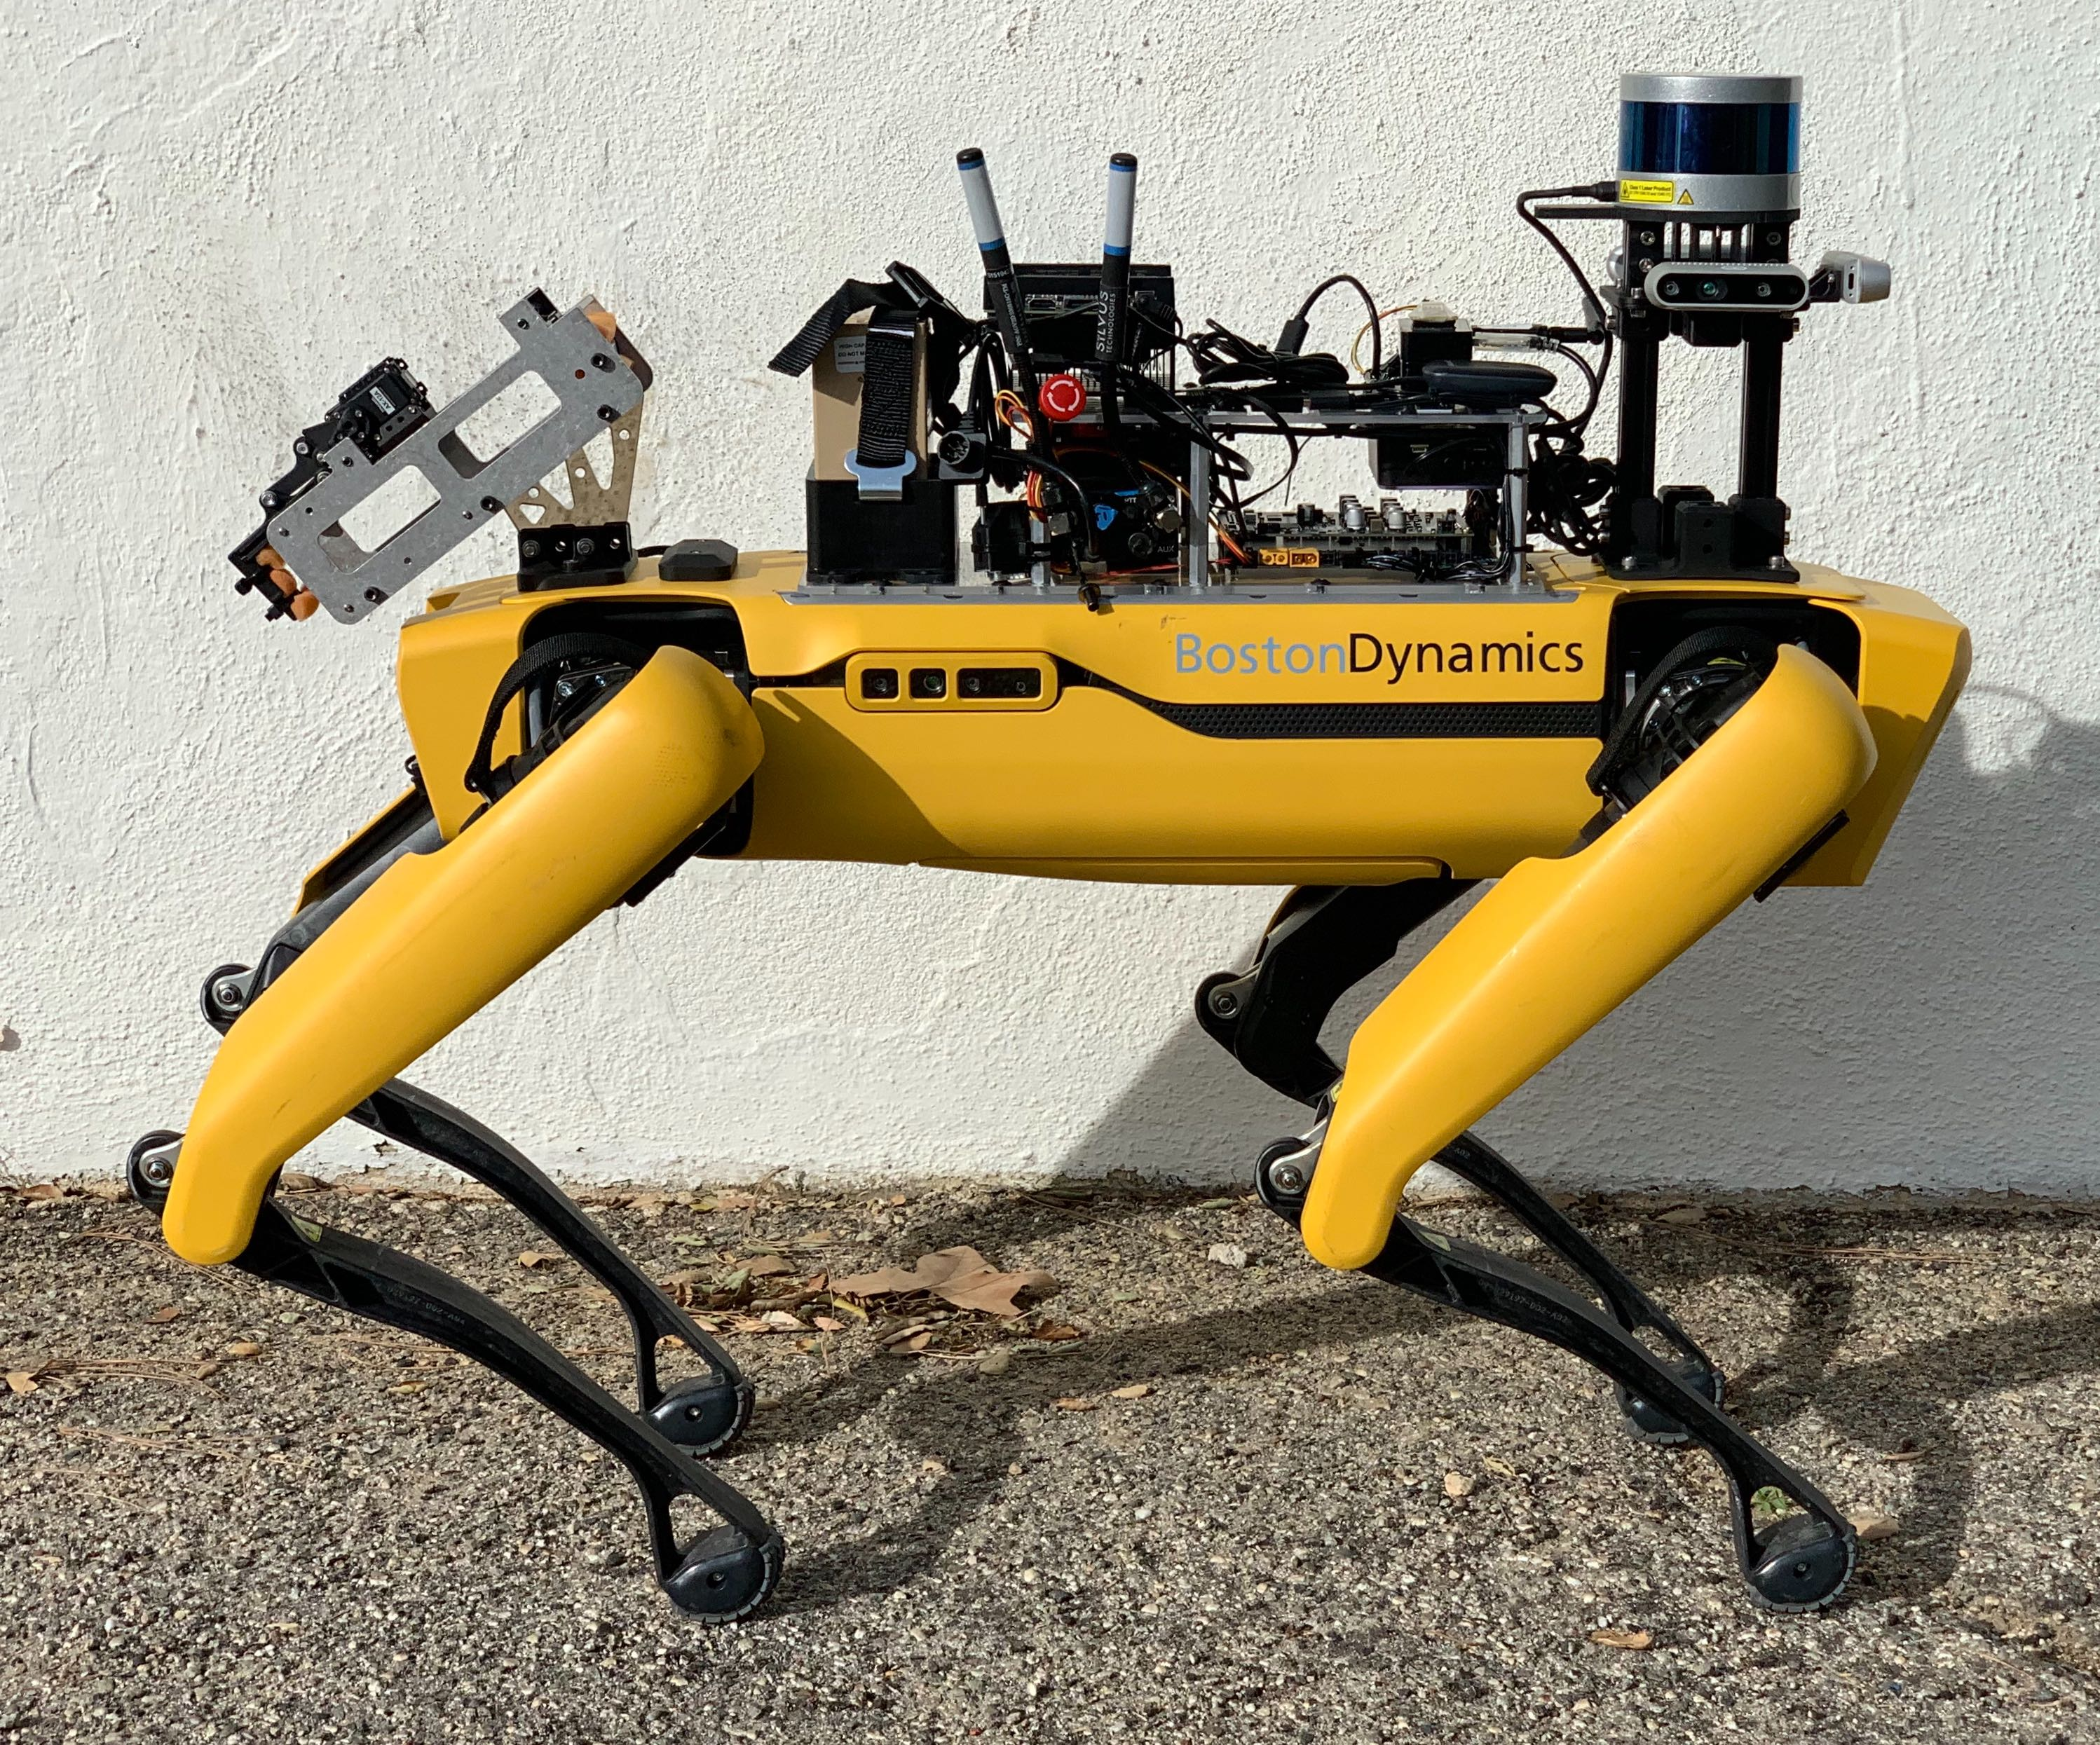
\includegraphics[width=0.3\textwidth]{spot_iros/graphics/spot_payload.jpg}
  \caption{\textbf{TODO:} One level IRM with behavior and frontier assignment marker. Like latetst Spot 161 autonomy test}
  \label{figurelabel}
\end{figure}


%%%%%%%%%%%%%%%%%%%%%%%%%%%%%%%%%%%%%%%%%%%
\subsection{Stair Climbing}
%%%%%%%%%%%%%%%%%%%%%%%%%%%%%%%%%%%%%%%%%%%
Spot demonstrated four successful stair climbing during the Urban Circuit scored runs. Each staircase consists of four flight of stairs with tight 180-degree turns in each landing. The stairs are metal-grated and approximately 0.27m in run, and 0.19m in rise. Figure \ref{fig:spot_stair_climb} shows a snapshot of Spot climbing down the stairs in the Alpha course.

Stair climbing operations pose challenges to odometry estimation because of frequent pitching motion,  slippages on the stair edges, and repetitive patterns. Figure \ref{fig:alpha_course_stairs_map} is a frontend map produced during the stair climbing operations. Although there is no ground-truth comparison yet, the fact that the artifact reports generated by the Spot are accepted for its classification and location is an indirect evidence that our odometry estimation is accurate.


\begin{figure}[t]
  \centering
  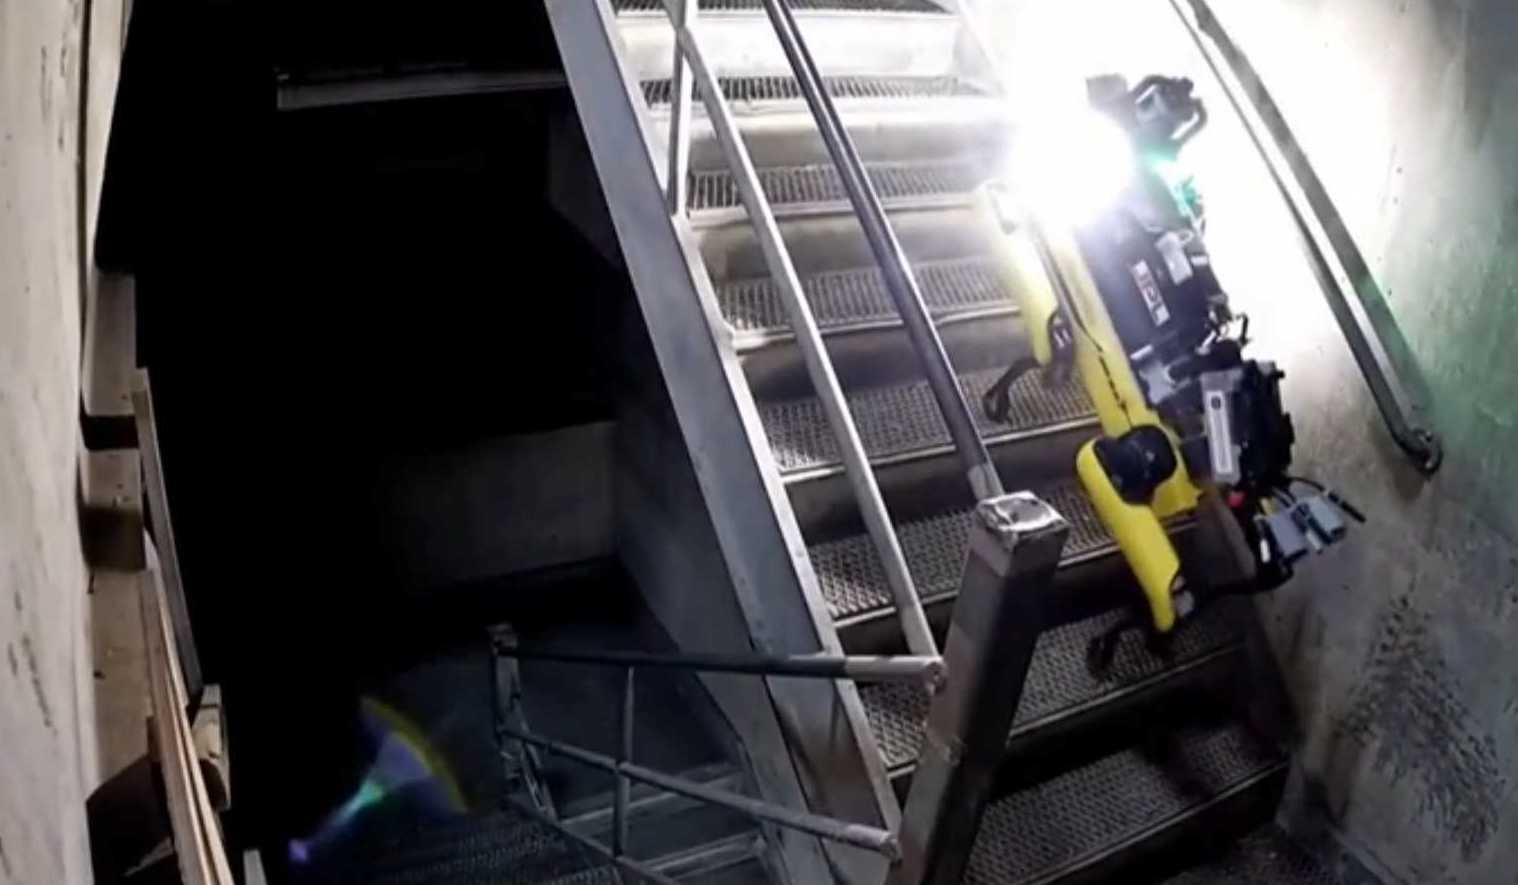
\includegraphics[width=0.45\textwidth]{spot_iros/graphics/spot_stairclimbing2.jpg}
  \caption{Spot stair climbing in Urban Circuit Alpha course.}
  \label{fig:spot_stair_climb}
\end{figure}

\begin{figure}[t]  % Moved from odometry section; Revert if necessary
  \centering
  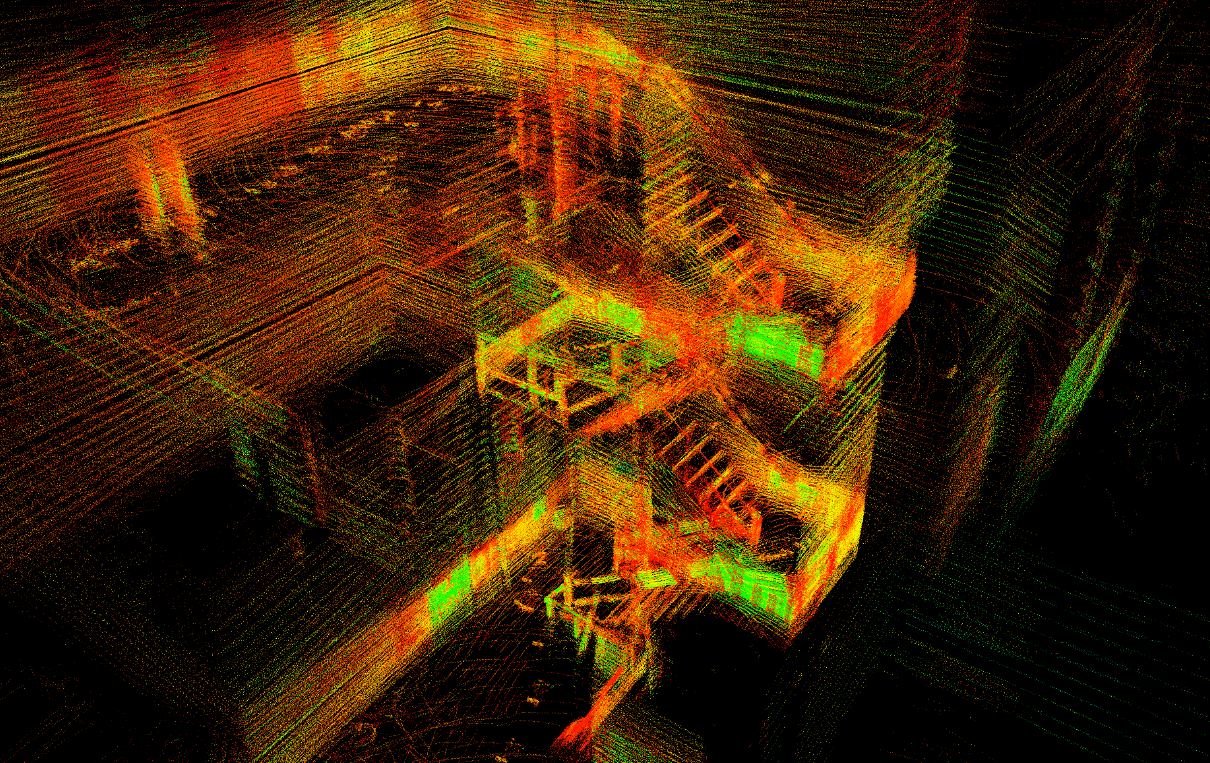
\includegraphics[width=0.45\textwidth]{spot_iros/graphics/spot_alpha_course_stairs.PNG}
  \caption{Spot Frontend map produced in Alpha Course}
  \label{fig:alpha_course_stairs_map}
\end{figure}



%%%%%%%%%%%%%%%%%%%%%%%%%%%%%%%%%%%%%%%%%%%
\subsection{Spot Operation in DARPA SubT Urban Circuit}
%%%%%%%%%%%%%%%%%%%%%%%%%%%%%%%%%%%%%%%%%%%

Two Spots are deployed in all four scored runs during the Urban Circuit. They traveled a combined distance of XX\,[km] in four runs, including four stair climbing of multiple flights of stairs. The Spots successfully detected XX artifacts from different levels, using RGB-D sensors, a thermal camera, a WiFi antenna, and a gas sensor. 

\inst{Lots of amazing pictures, accuracy of localization, traversability
Images of: Spot in extreme terrain, LAMP Map, IRM, Comms map, Comm dropping, Stair Climbing}

\newpage

%%%%%%%%%%%%%%%%%%%%%%%%%%%%%%%%%%%%%%%%%%%
\section{Lessons Learned and Future Directions}\label{sec:conclusion}
%%%%%%%%%%%%%%%%%%%%%%%%%%%%%%%%%%%%%%%%%%%
% Robosimian's journal intro sentences of lessons learned
This section summarizes some of the highlights of our platform,
discusses the lessons learned, and justifies the core
assumptions we made in design, testing, and operations:
% I think its not in order yet

% Fadhil. May be this subsection can be moved to Robot behaviors?
\subsection{Recovery}
Due to the challenging terrain of Spot at the test area, we consider a possibility that the robot might fall.
%
Fortunately, Spot has ability to "SELFRIGHT" itself from falling to sitting position and still operational after that.
%
However, on some cases, we find that the robot is not able to stand up after a successful "SELFRIGHT" because the legs placement are not stable after the recovery.
%
As a work around to robustify the behaviors in the current Spot software that we use, we send a repetitive command of quick stand and sit to improve better placement of the legs.

\subsection{Traversability}
Currently, traversability is purely defined geometrically (obstacles, slopes, holes,...).
However, when traversing challenging terrains, as encountered in the SubT challenge, the notion of traversability has to be extended.
While there are many metrics, which can be considered for traversability and that have been described by Papadakis in \cite{Papadakis2013}, the most important one would be surface friction.
Due to small contact surface and, compared to wheeled or tracked robots, and dynamic gaits, quadrupeds suffer more from slippery surfaces such as wet or dusty surfaces. 

For this reason, traversability has to include surface friction informations so that it can be avoided by the local planner, if possible.
If avoidance should not be possible, this information could at least be used to adaptively set the surface friction coefficient, which is used by the Spot's internal planner.

Another traversability metric might include terramechanics in order to avoid soft soil, where the feet of the robot might sink in.

Another traversability metric might be to not step on movable items (loose plates or things on which Spot crashed)

=> We need traversability from semantic scene understanding, not just geometric anymore!!!

\inst{This kind of discussion should go to the experiment section. - This does not fit the method section} The Nebula global planner, which is described in more detail in Section \ref{sec:mission_planning}, can select goals up to 10 meters away from the current robot's position.
However, Spot's internal planner works with a 4x4 m map of the environment.
Even though, waypoints outside of the internal map can be given to the internal planner, this caused some issues such as the robot taking sub--optimal paths or not avoiding some obstacles such as overhangs, cliffs or obstacles within the blind spots of the internal sensors.
Because, the Nebula payload offers more sensing capabilities, especially due to the long--range sensors such as the LiDAR, we chose to add an intermediate planner in order to bridge the gap and avoid and complement the Spot internal planner.

======

\subsection{Perception--Aware Planning}
Legged robots, such as Spot, have a higher degree--of--freedom than most ground robots, which usually have a fixed chassis.
This higher level of configurability decouples the robot's overall motion from the floating base's attitude to a certain extent.
One interesting direction would be to exploit this characteristic of the floating base for perception--aware planning.
For example by pitching or rolling the robot's base in order to maximize sensor coverage and reduce blind spots.

====

We have access to BD costmap and additional obstacle information, which spot might not see. When giving global waypoints (far away), the robot might not be able to avoid some of these or end up taking suboptimal paths due to the small costmap (4x4m). We plan intermediate waypoints (with Dijkstra) to avoid this problem. Additionally, we prefer forward motion due to sensor coverage (blind spot avoidance and artifact detection), so we choose the waypoint heading in a way which encourages the robot to go forward. Waypoints are given to Spot's internal planner, which then executes the actual trajectory.

Mentio that, even though we can try to avoid these regions by not giving waypoints in that region we cannot guarantee that BD will actually avoid these regions.

Define, how we assign an orientation to the previously selected waypoint in order to bias forward motion


\subsection{Intelligent Behaviour Selection}
Automatics stair detection and climbing, changing gaits (crawl) to get over rubble,...)
BD offers a very limited, but powerful, set of tuning knobs (gait, stair mode, surface friction, body height,...).
However, these are either set to fixed average values or chosen by the human supervisor.
One push would be to switch and set these tuning knobs autonomously (for example choose gait based on what the long range sensors see, set surface friction by estimating surface friction, autonomously change to stair mode and do autonomous stair climbing instead of human given wp)


\subsection{Collaboration}
Spot as drone carrier?
\subsection{}
%%%%%%%%%%%%%%%%%%%%%%%%%%%%%%%%%%%%%%%%%%%
\section{CONCLUSIONS}
%%%%%%%%%%%%%%%%%%%%%%%%%%%%%%%%%%%%%%%%%%%



\addtolength{\textheight}{-12cm}   % This command serves to balance the column lengths
                                  % on the last page of the document manually. It shortens
                                  % the textheight of the last page by a suitable amount.
                                  % This command does not take effect until the next page
                                  % so it should come on the page before the last. Make
                                  % sure that you do not shorten the textheight too much.

%%%%%%%%%%%%%%%%%%%%%%%%%%%%%%%%%%%%%%%%%%%%%%%%%%%%%%%%%%%%%%%%%%%%%%%%%%%%%%%%



%%%%%%%%%%%%%%%%%%%%%%%%%%%%%%%%%%%%%%%%%%%%%%%%%%%%%%%%%%%%%%%%%%%%%%%%%%%%%%%%



%%%%%%%%%%%%%%%%%%%%%%%%%%%%%%%%%%%%%%%%%%%%%%%%%%%%%%%%%%%%%%%%%%%%%%%%%%%%%%%%
\section*{APPENDIX}

Appendixes should appear before the acknowledgment.

\section*{ACKNOWLEDGMENT}
The research was carried out at the Jet Propulsion Laboratory, California Institute of Technology, under a contract with the National Aeronautics and Space Administration. This work was partially funded by the Defense Advanced Research Projects Agency (DARPA). Government Sponsorship acknowledged.



%%%%%%%%%%%%%%%%%%%%%%%%%%%%%%%%%%%%%%%%%%%%%%%%%%%%%%%%%%%%%%%%%%%%%%%%%%%%%%%%


%%%%%%%%%%%%%%%%%%%%%%%%%%%%%%%%%%%%%%%%%%%
%%%%%%%%%%%%%%%%%%%%%%%%%%%%%%%%%%%%%%%%%%%
\bibliographystyle{IEEEtran}
\bibliography{main}
%%%%%%%%%%%%%%%%%%%%%%%%%%%%%%%%%%%%%%%%%%%
\end{document}


